%!TEX root = main.tex
\section{Motivating Examples}
\label{sec:motivation}

%TODO GIVE AN EXAMPLE FOR 1 ROBUSTNESS AND 2 ROBUSTNESS IN THE P LANGUAGE (EXPLAIN A LITTLE BIT THE SYNTAX)
%
%TALK ABOUT THE MOST USUAL WAY OF SEEING THEM
%
%TAKE SOME EXECUTIONS AND SHOW HOW THEY CAN BE REORDERED AND EXECUTED ON A STRONGER SEMANTICS
%
%EXPLAIN THE STRONGER SEMANTICS
%
%SAY THAT FINDING VIOLATIONS MEANS DETECTING SOME PARTICULAR CLASS OF CYCLES
%
%SAY WHAT ARE THE CONSEQUENCES: SAFETY, DEADLOCK
%
%SAY THAT FINDING SUCH CYCLES CAN BE DONE ON THE STRONGER SEMANTICS - GIVE THE MAIN IDEAS

We provide in this section examples illustrating the relevance and the applicability of our approach. %These examples correspond to several types of protocols used in practice. 
Figure~\ref{fig:commit} shows a {\em commit protocol} allowing a client to update a memory that is replicated in two processes, called \emph{nodes}. The access to the nodes is controlled by a manager. Figure~\ref{fig:commit-exec} shows an execution of this protocol. This system is 1-synchronizable, i.e., every execution is equivalent to one where only rendezvous communication is used. Intuitively, this holds because mutually interacting components are never in the situation where messages sent from one to the other are crossing messages sent in the other direction (i.e., the components are "talking" to each other at the same time). For instance, the execution in Figure~\ref{fig:commit-exec} is 1-synchronizable because its \emph{conflict graph} (shown in the same figure) is acyclic. Nodes in the conflict graph are matching send-receive pairs (numbered from 1 to 6 in the figure), and edges correspond to the program order between actions in these pairs. The label of an edge records whether the actions related by program order are sends or receives, e.g., the edge from 1 to 2 labeled by $RS$ represents the fact that the receive of the send-receive pair 1 is before the send of the send-receive pair 2, in program order. For the moment, these labels should be ignored, their relevance will be discussed in Section~\ref{sec:characterizations}.
The conflict graph being acyclic means that matching pairs of send-receive actions are ``serializable'', which implies that this execution is equivalent to one where every send is immediately followed by the matching receive (as in rendezvous communication).

\begin{figure}[t]
\begin{center}
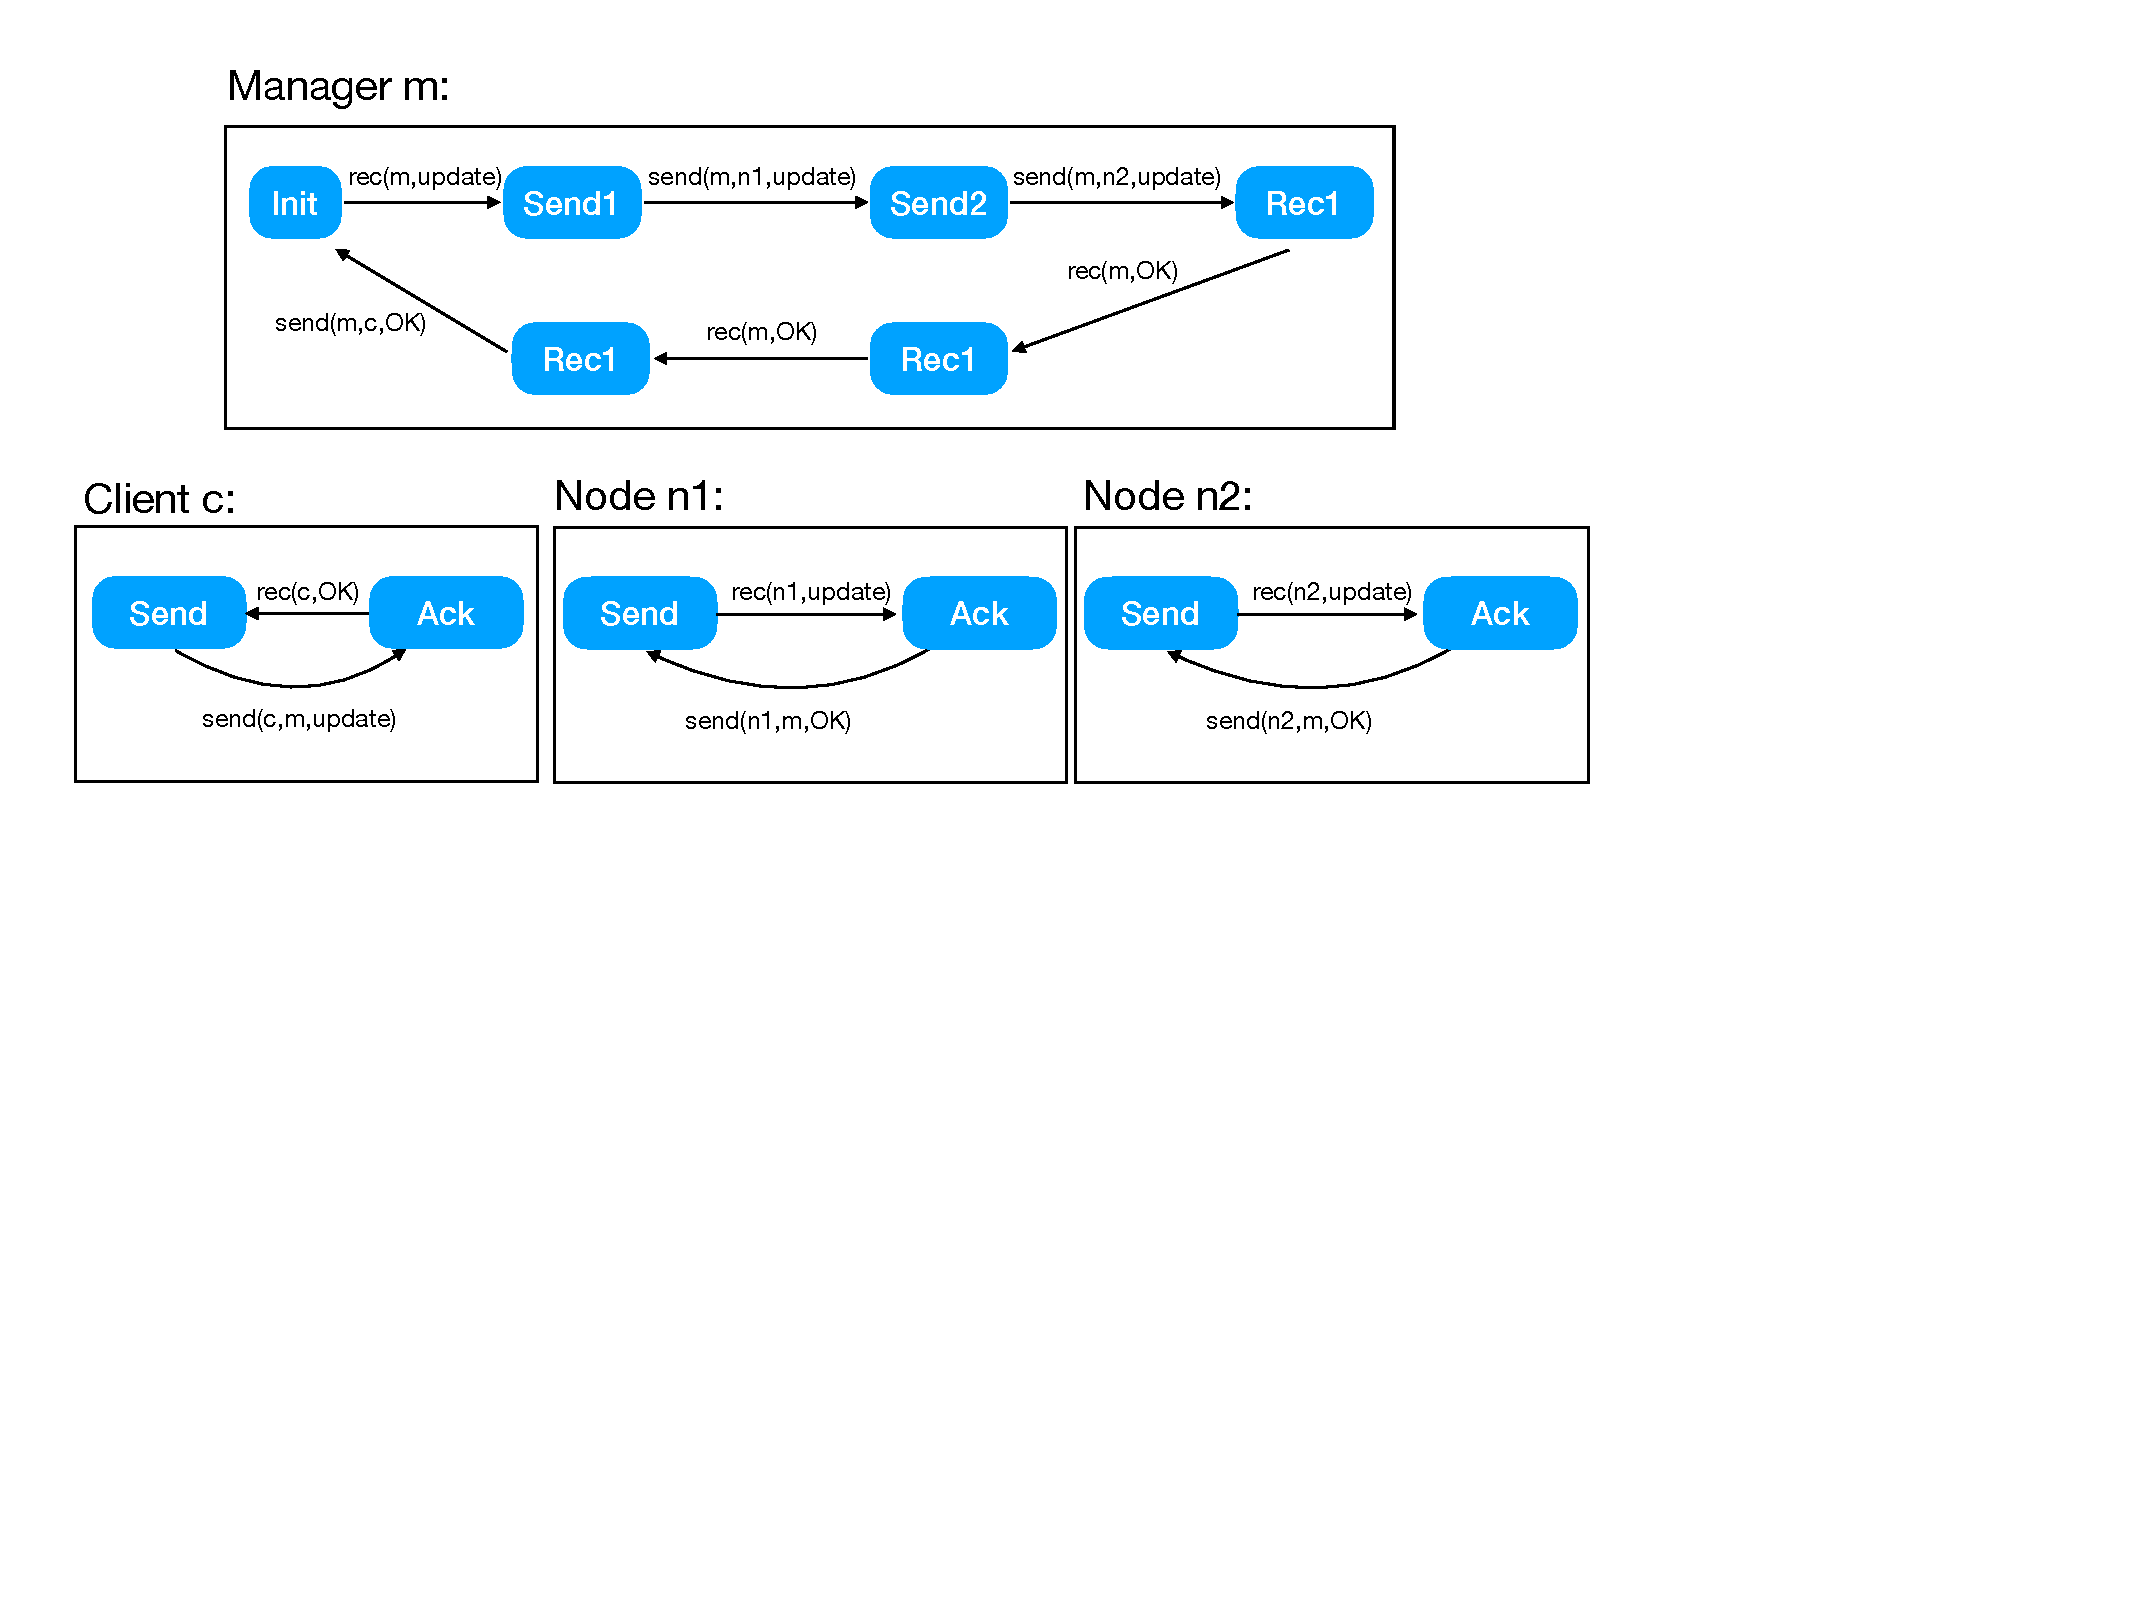
\includegraphics[width=8.5cm]{commit.pdf}
\end{center}
\vspace{-5.5mm}
\caption{A distributed commit protocol. Each process is defined as a labeled transition system. Transitions are labeled by send and receive actions, e.g., $\senda{\sf{c},\sf{m},\sf{update}}$ is a send from the client $\sf{c}$ to the manager $\sf{m}$ with payload $\sf{update}$. Similarly, $\reca{c,\sf{OK}}$ denotes process $\sf{c}$ receiving a message 
$\sf{OK}$.}
\label{fig:commit}
\vspace{-3.5mm}
\end{figure}

\begin{figure}[t]
\begin{center}
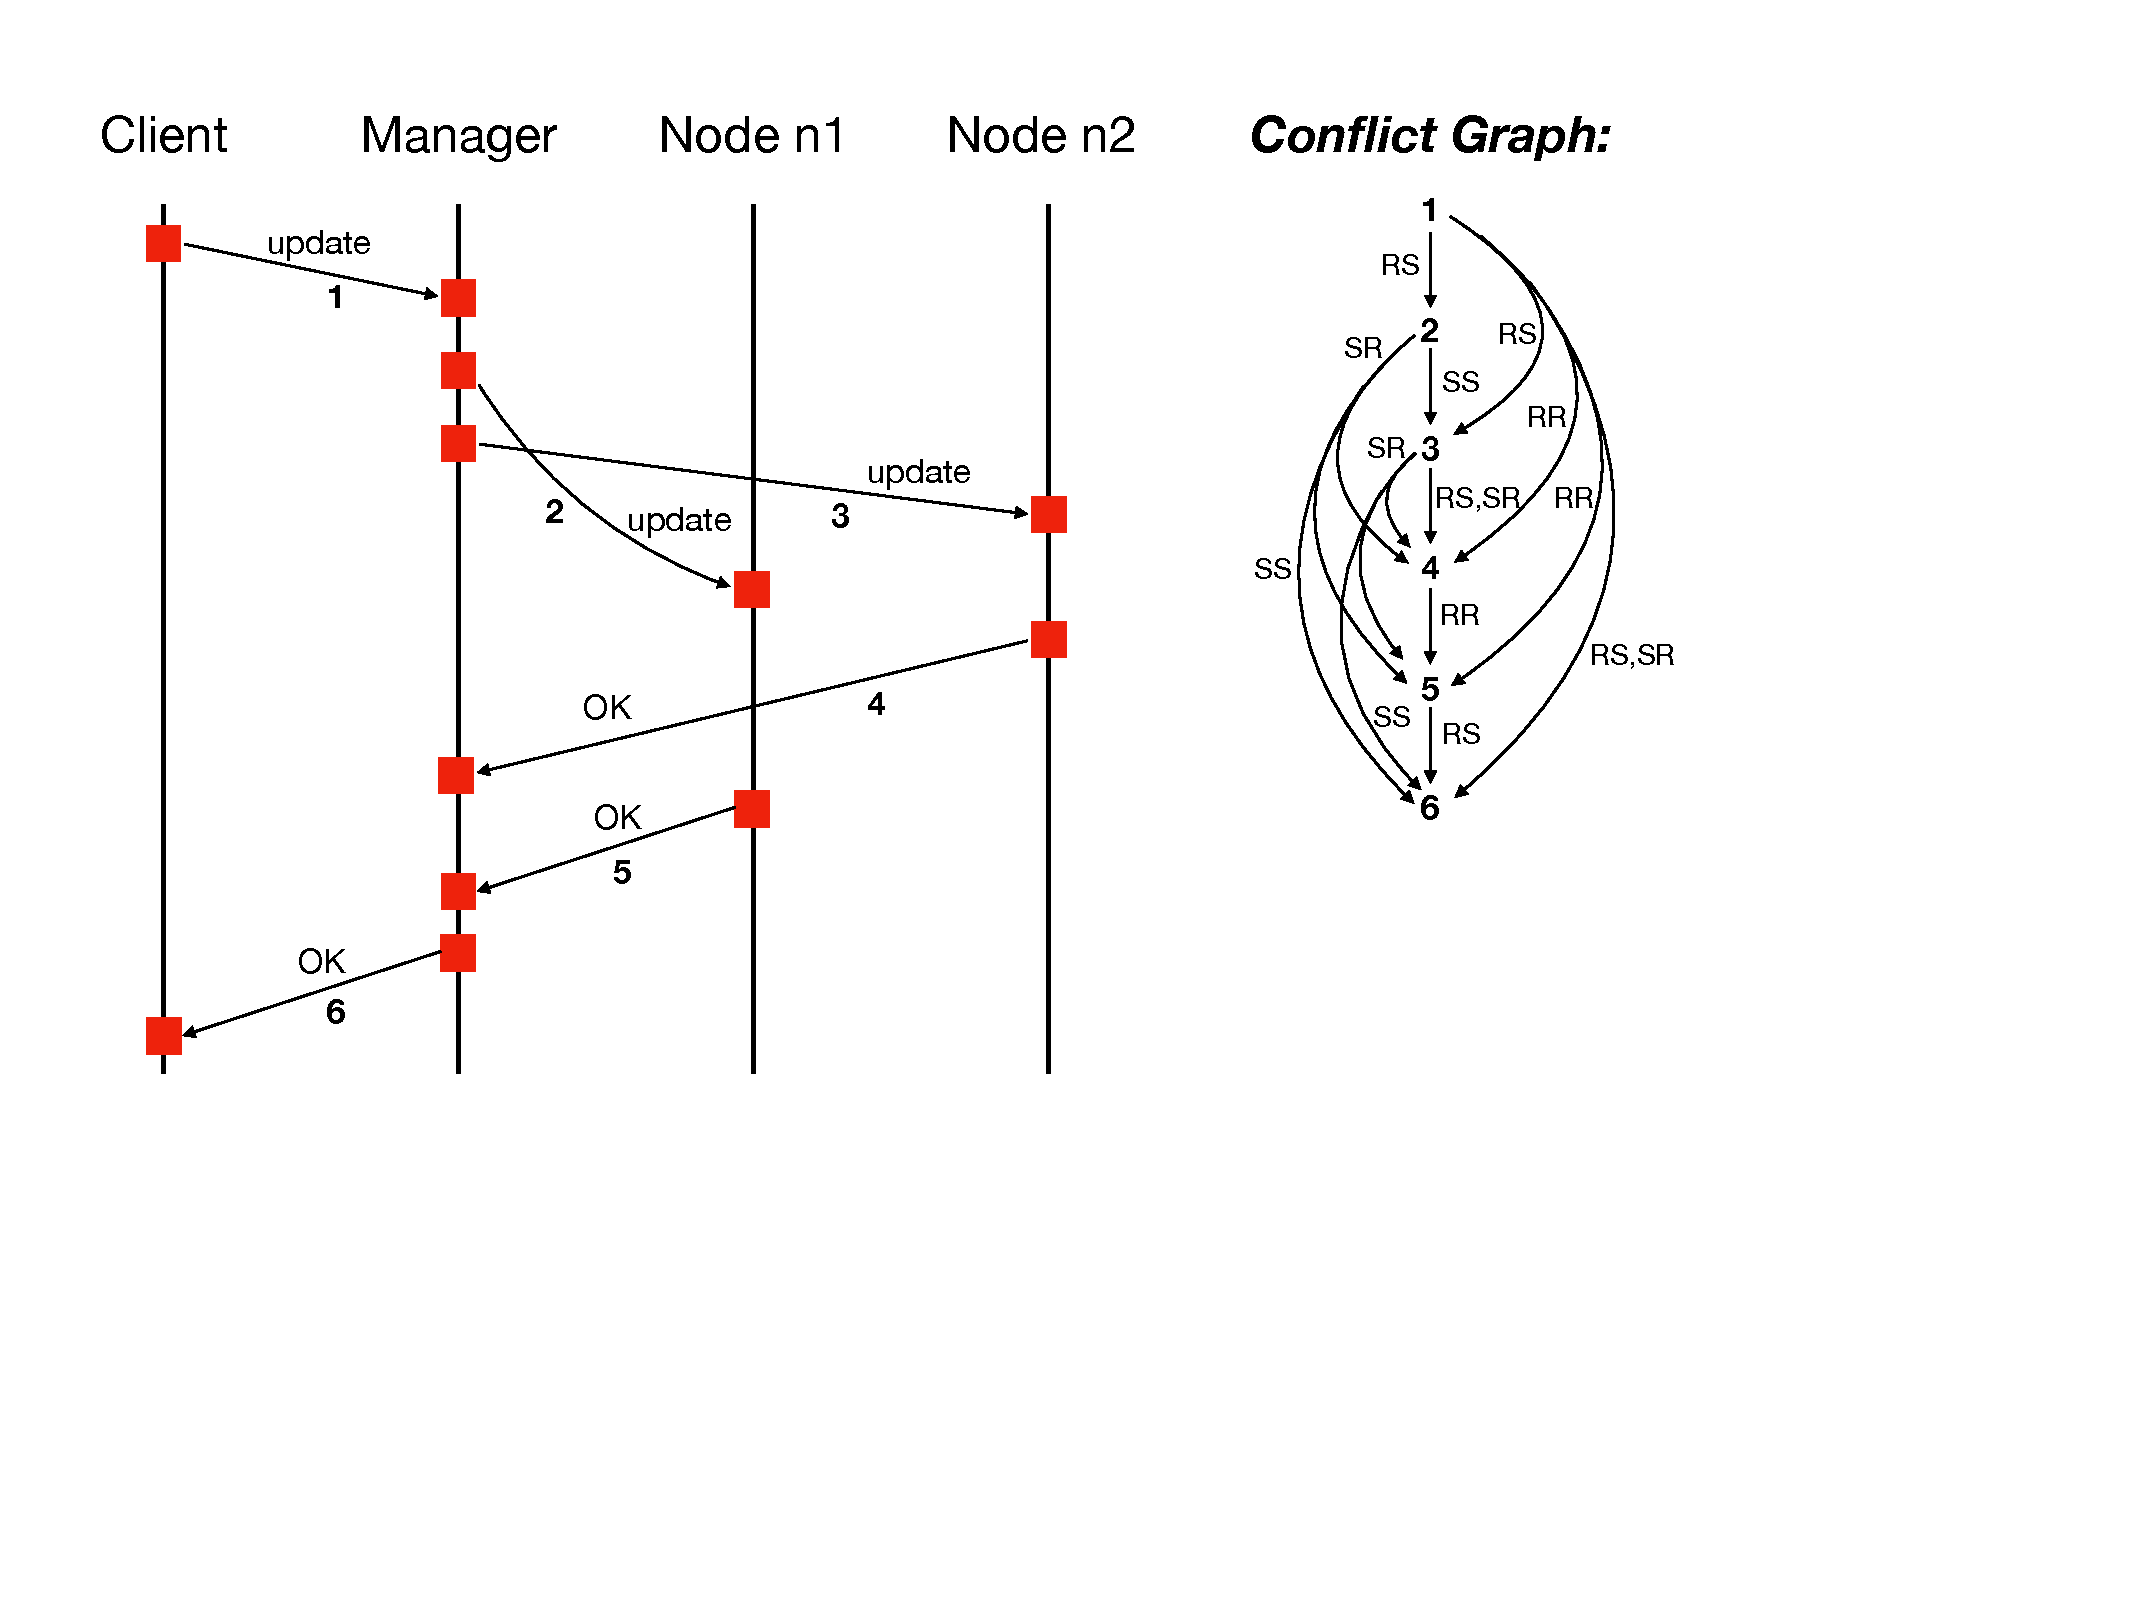
\includegraphics[width=7cm]{MSC-commit.pdf}
\end{center}
\vspace{-5mm}
\caption{An execution of the distributed commit protocol and its conflict graph.}
\label{fig:commit-exec}
\vspace{-7mm}
\end{figure}

Although the message buffers are bounded in all the computations of the commit protocol, this is not true for every 1-synchronizable system.
%Now, it can be observed that in the commit protocol message buffers are bounded in all the possible computations. This is in general not the case for 1-synchronizable systems. It might be the case indeed that 
There are asynchronous computations where buffers have an arbitrarily big size, which are equivalent to synchronous computations. This is illustrated by a (family of) computations shown in Figure~\ref{fig:elevator-exec1} of the system modeling an elevator described in Figure \ref{fig:elevator} (a simplified version of the system described in~\cite{DBLP:conf/pldi/DesaiGJQRZ13}). This system consists of three processes: {\sf User} models the user of the elevator, {\sf Elevator} models the elevator's controller, and {\sf Door} models the elevator's door which reacts to commands received from the controller. 
The execution in Figure~\ref{fig:elevator-exec1} models an interaction where the user sends an unbounded number of requests for closing the door, which generates an unbounded number of messages in the entry buffer of {\sf Elevator}. These computations are 1-synchronizable since they are equivalent to a 1-synchronous computation where {\sf Elevator} receives immediately every message sent by {\sf User}. This is witnessed by the acyclicity of the conflict graph of this computation (shown on the right of the same figure). It can be checked that the elevator system without the dashed edge is a 1-synchronous system. 

Consider now a slightly different version of the elevator system where the transition from {\sf Stopping2} to {\sf Opening2} is moved to target {\sf Opening1} instead (see the dashed transition in Figure \ref{fig:elevator}). It can be seen that this version reaches exactly the same set of configurations (tuples of process local states) as the previous one. Indeed, modifying that transition enables {\sf Elevator} to send a message {\sf open} to {\sf Door}, but the latter can only be at {\sf StopDoor}, {\sf OpenDoor}, or {\sf ResetDoor} at this point, and therefore it can (maybe after sending {\sf doorStopped} and {\sf doorOpened}) receive at state {\sf ResetDoor} the message {\sf open}. However, receiving this message doesn't change {\sf Door}'s state, and the set of reachable configurations of the system remains the same. This version of the system is not 1-synchronizable as it is shown in Figure \ref{fig:elevator-exec2}: once the {\sf doorStopped} message sent by {\sf Door} is received by {\sf Elevator}~\footnote{{\sf Door} sends the message from state {\sf StopDoor}, and {\sf Elevator} is at state {\sf Stopping2} before receiving the message.}, these two processes can send messages to each other at the same time (the two send actions happen before the corresponding receives). This mutual interaction consisting of 2 parallel send actions is called a \emph{$2$-exchange} and it is witnessed by the cycle of size 2 in the execution's conflict graph (shown on the right of Figure \ref{fig:elevator-exec2}).
%Suppose that {\sf Door} is at state {\sf StopDoor}, and that {\sf Elevator} is at state {\sf Stopping2}. Then, {\sf Door} can send a message {\sf doorStoped} and move to the state {\sf OpenDoor}. Next, {\sf Elevator} can receive that message and move to state {\sf Opening1}. At this point, {\sf Elevator} and {\sf Door} can only exchange messages: message {\sf doorOpened} from {\sf Door} to {\sf Elevator} and message {\sf open} from {\sf Elevator} to {\sf Door}. 
In general, it can be shown that every execution of this version of the elevator system has a conflict graph with cycles of size at most 2, which implies that it is 2-synchronizable (by the results in Section~\ref{sec:characterizations}).

\begin{figure}[t]
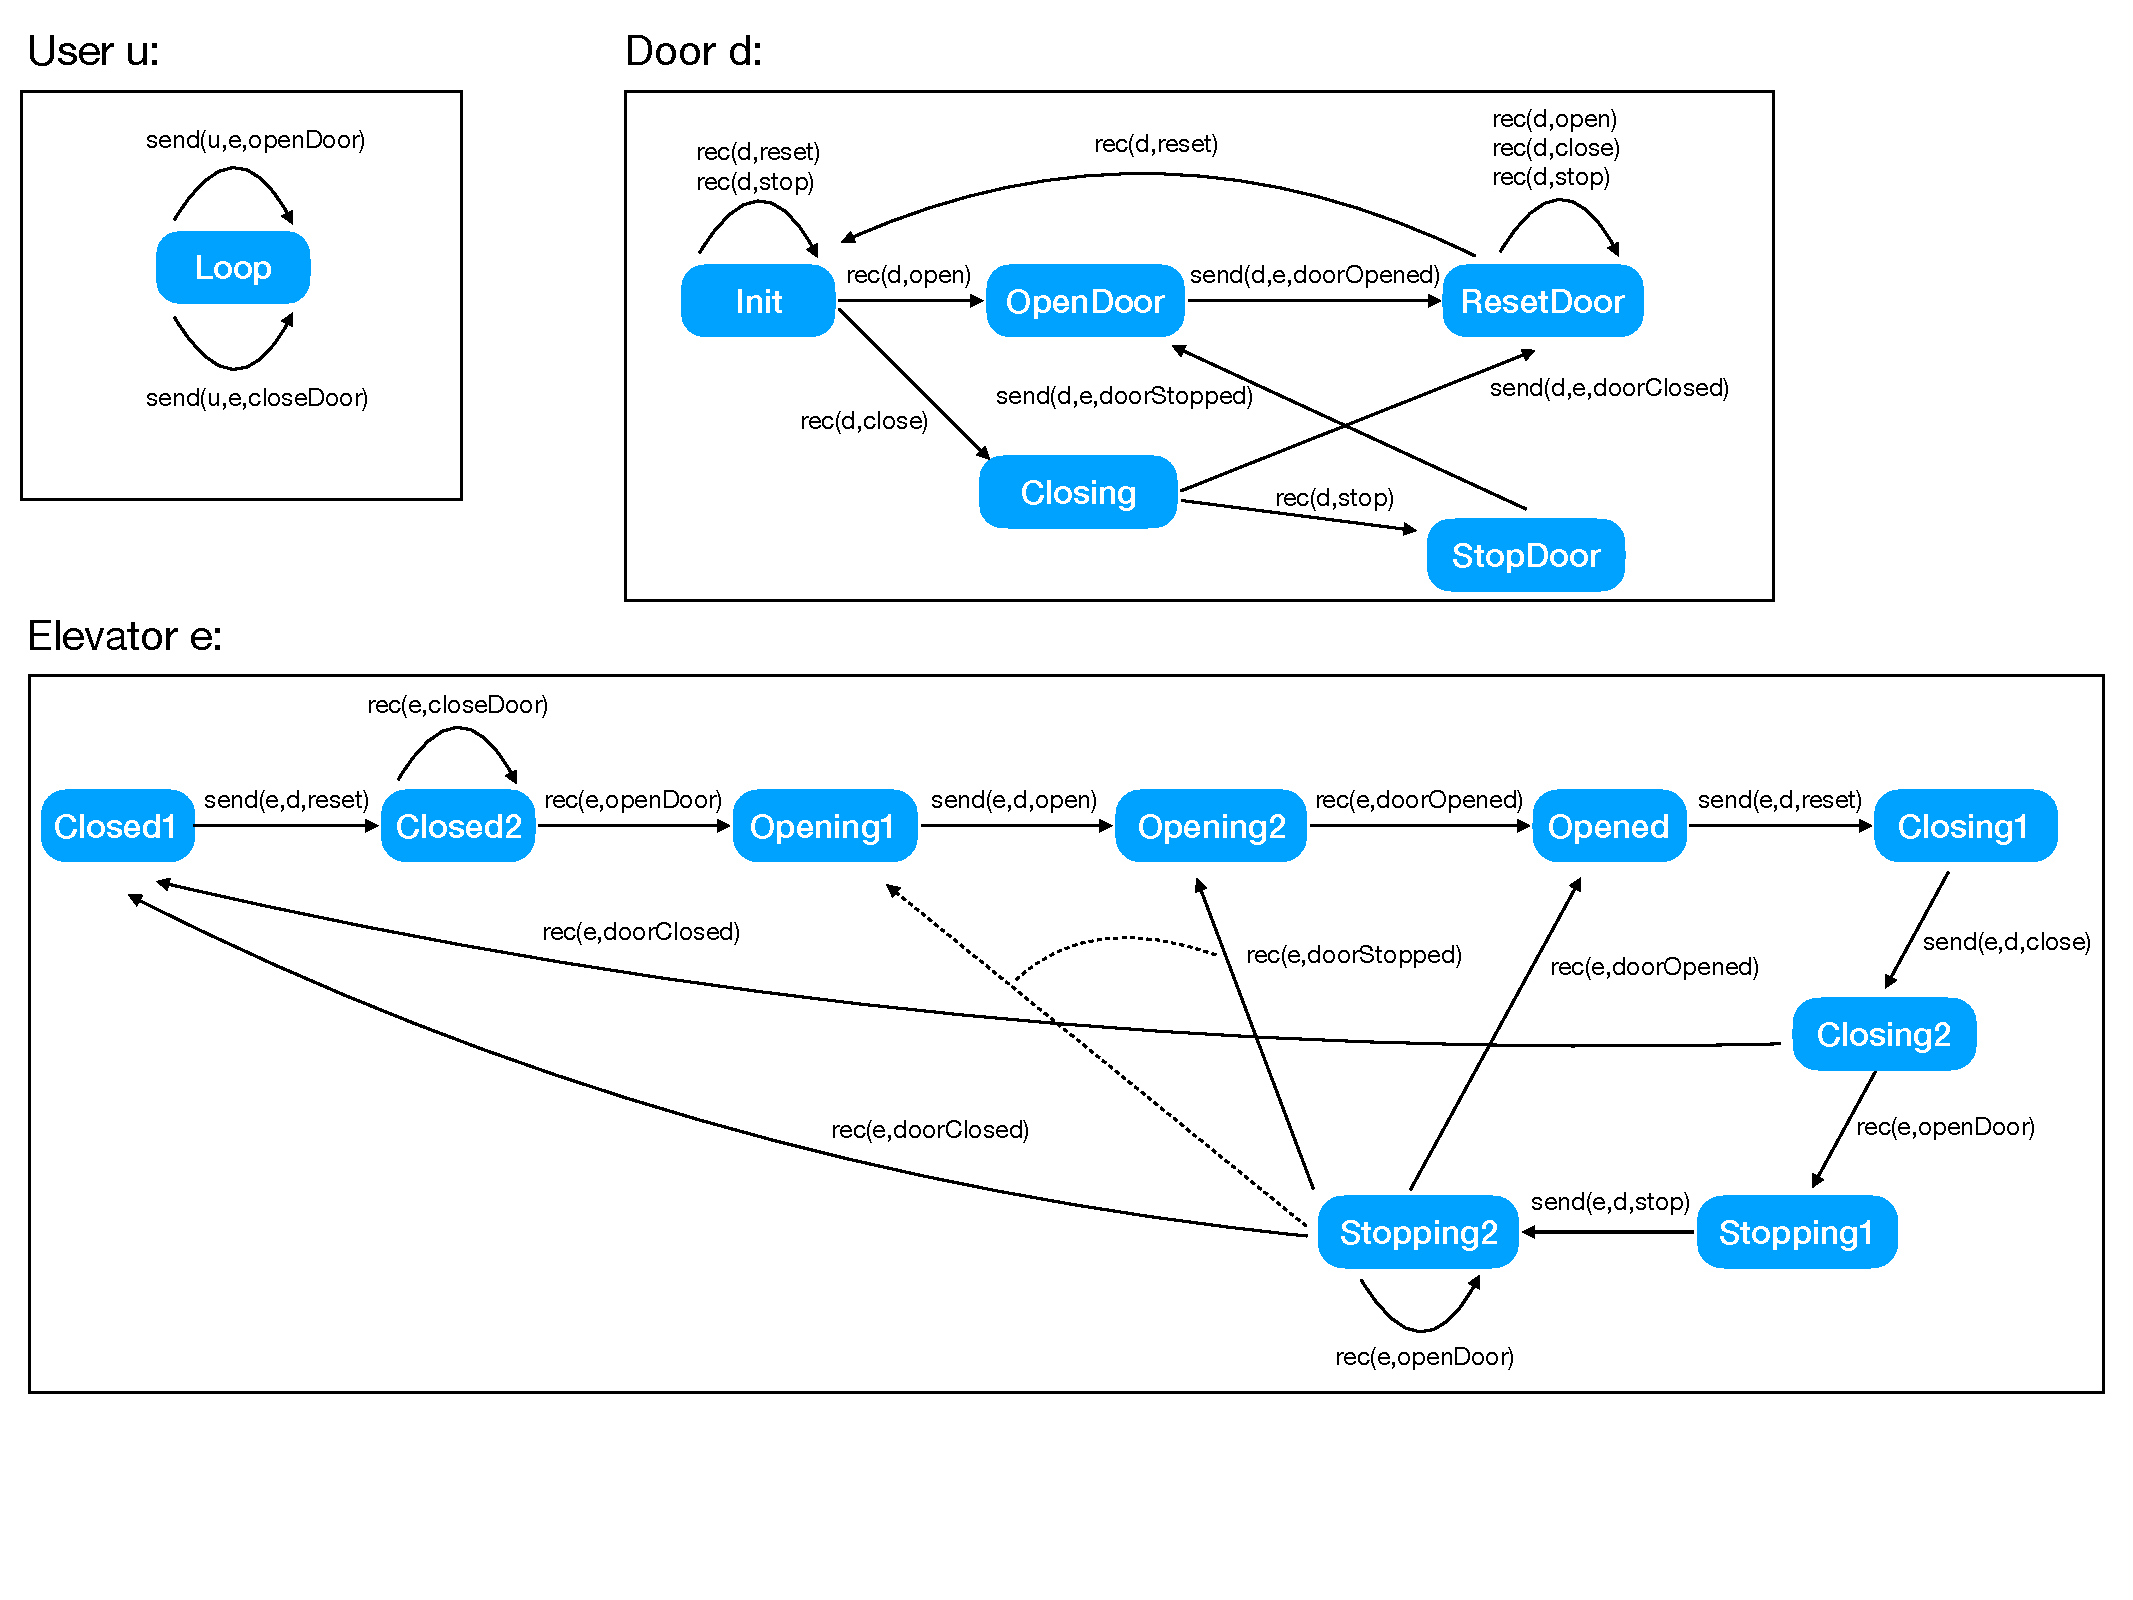
\includegraphics[width=12cm]{elevator.pdf}
\vspace{-3mm}
\caption{A system modeling an elevator.}
\label{fig:elevator}
\vspace{-5mm}
\end{figure}

\begin{figure}[t]
\begin{subfigure}[t]{5.2cm}
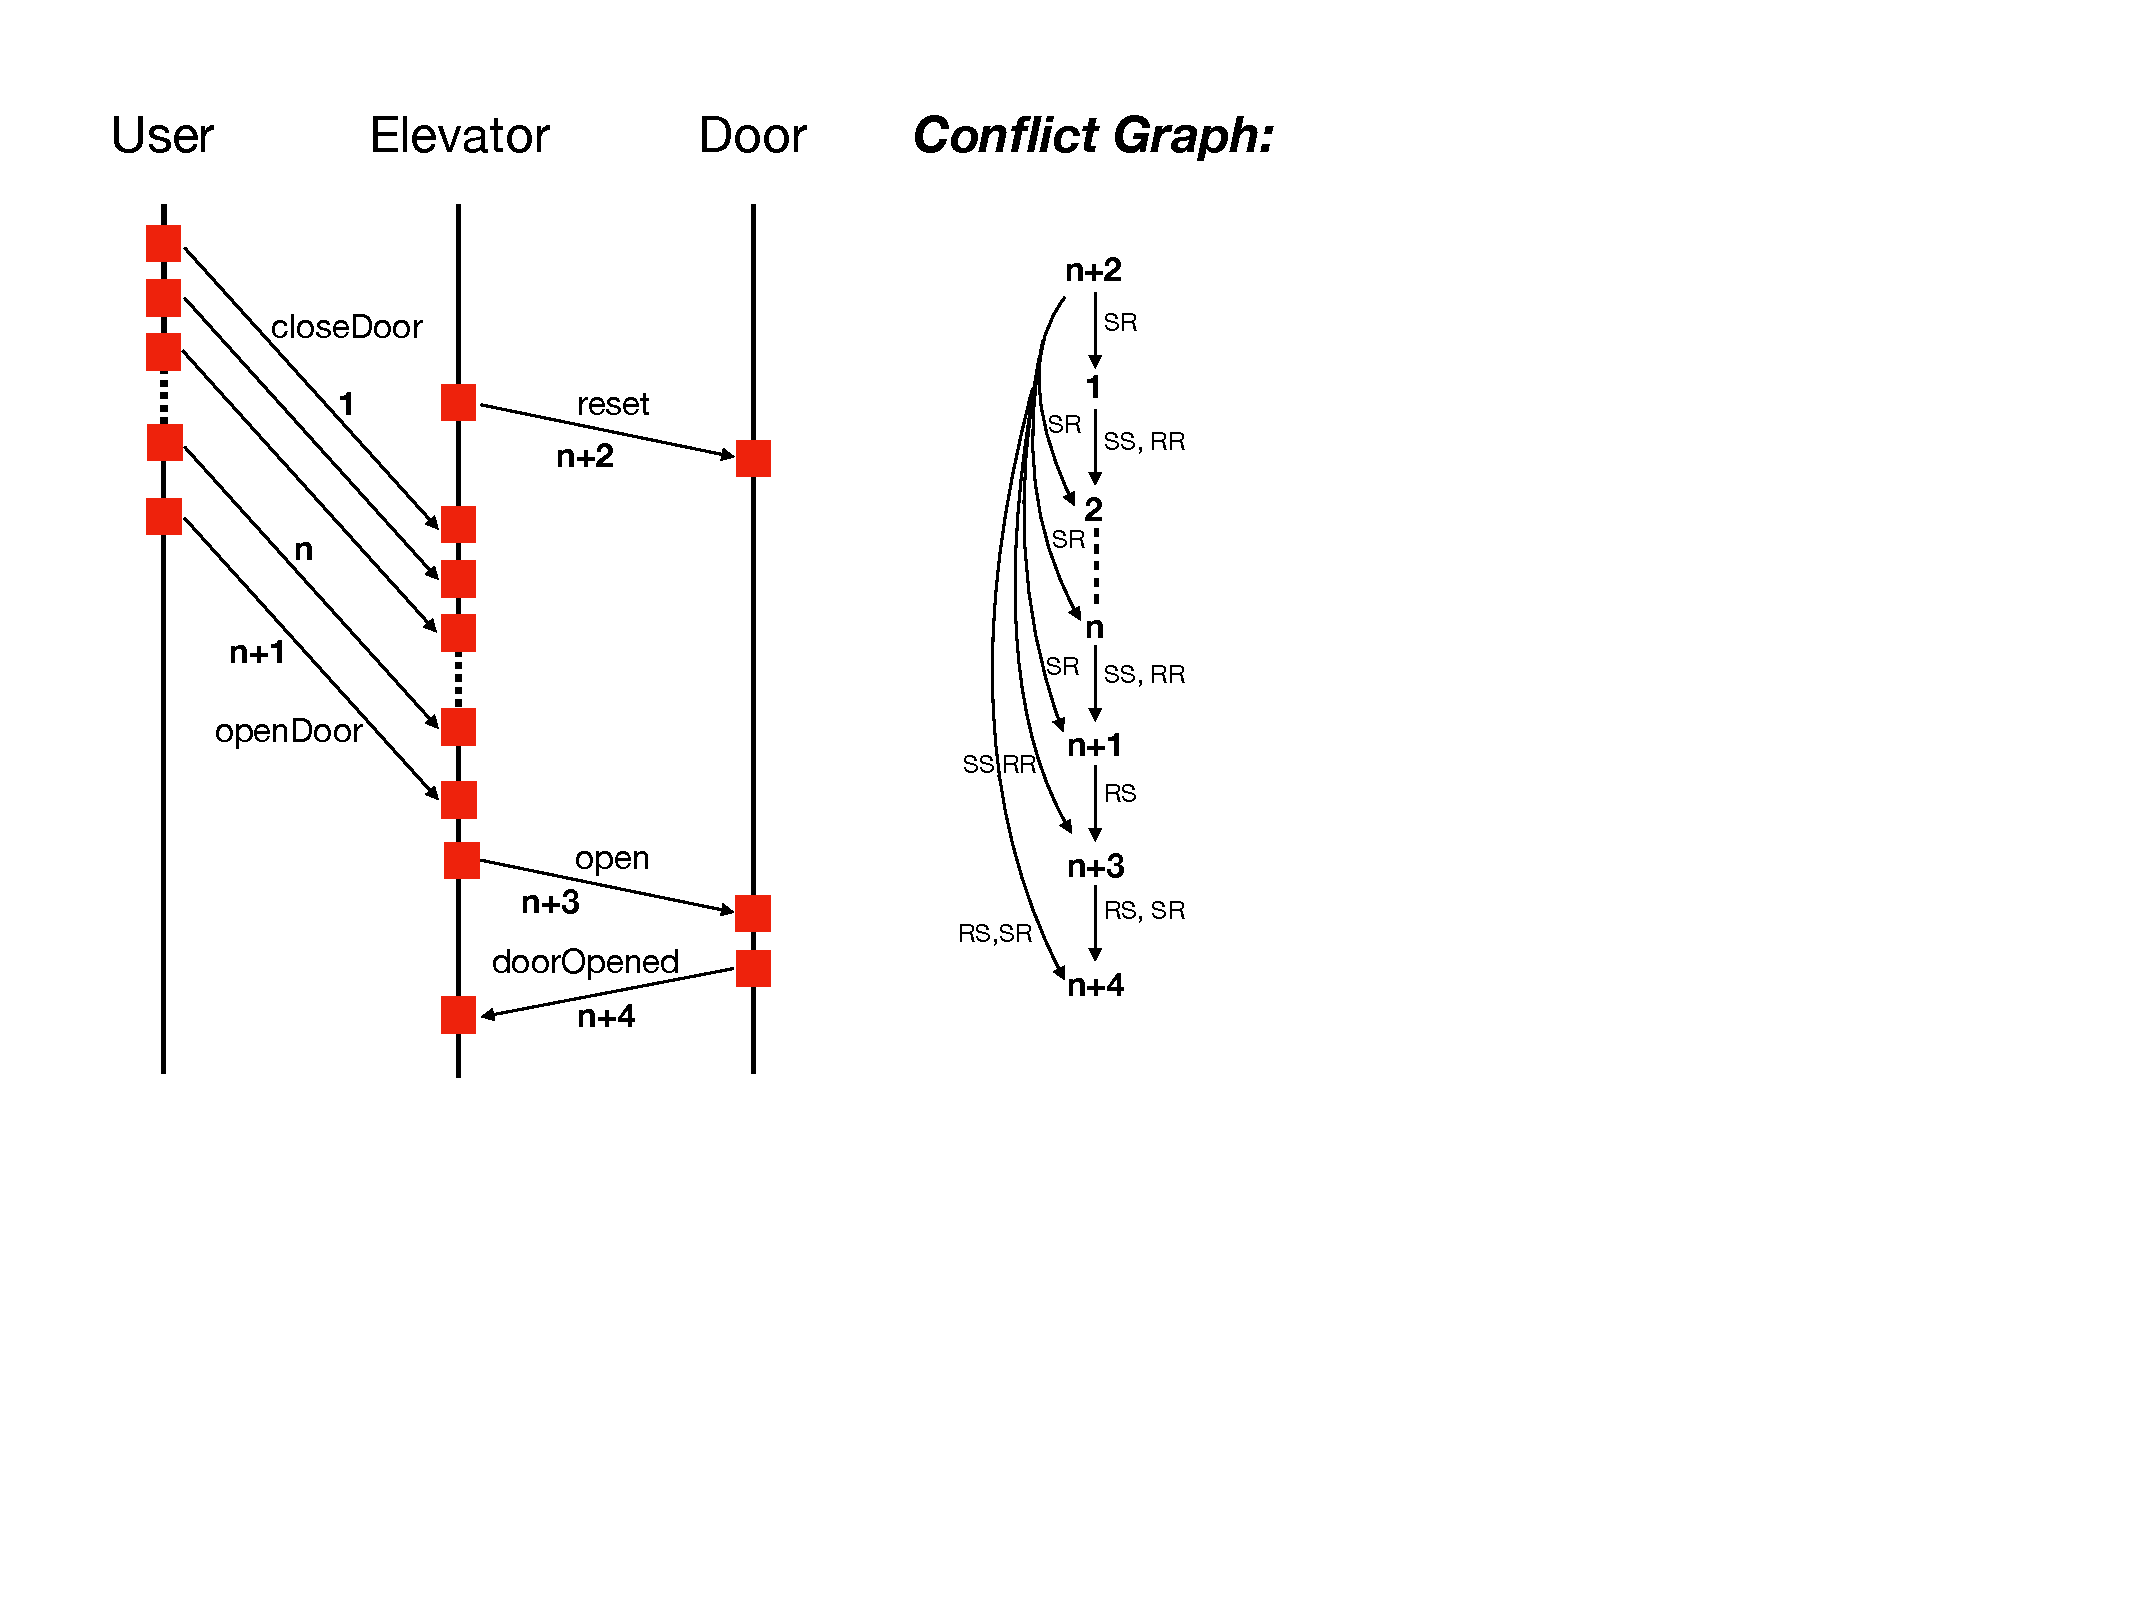
\includegraphics[width=6cm]{MSC-elevator1.pdf}
\vspace{-3mm}
\caption{A $1$-synchronizable execution.}
\label{fig:elevator-exec1}
\end{subfigure}
\hspace{1cm}
\begin{subfigure}[t]{5.5cm}
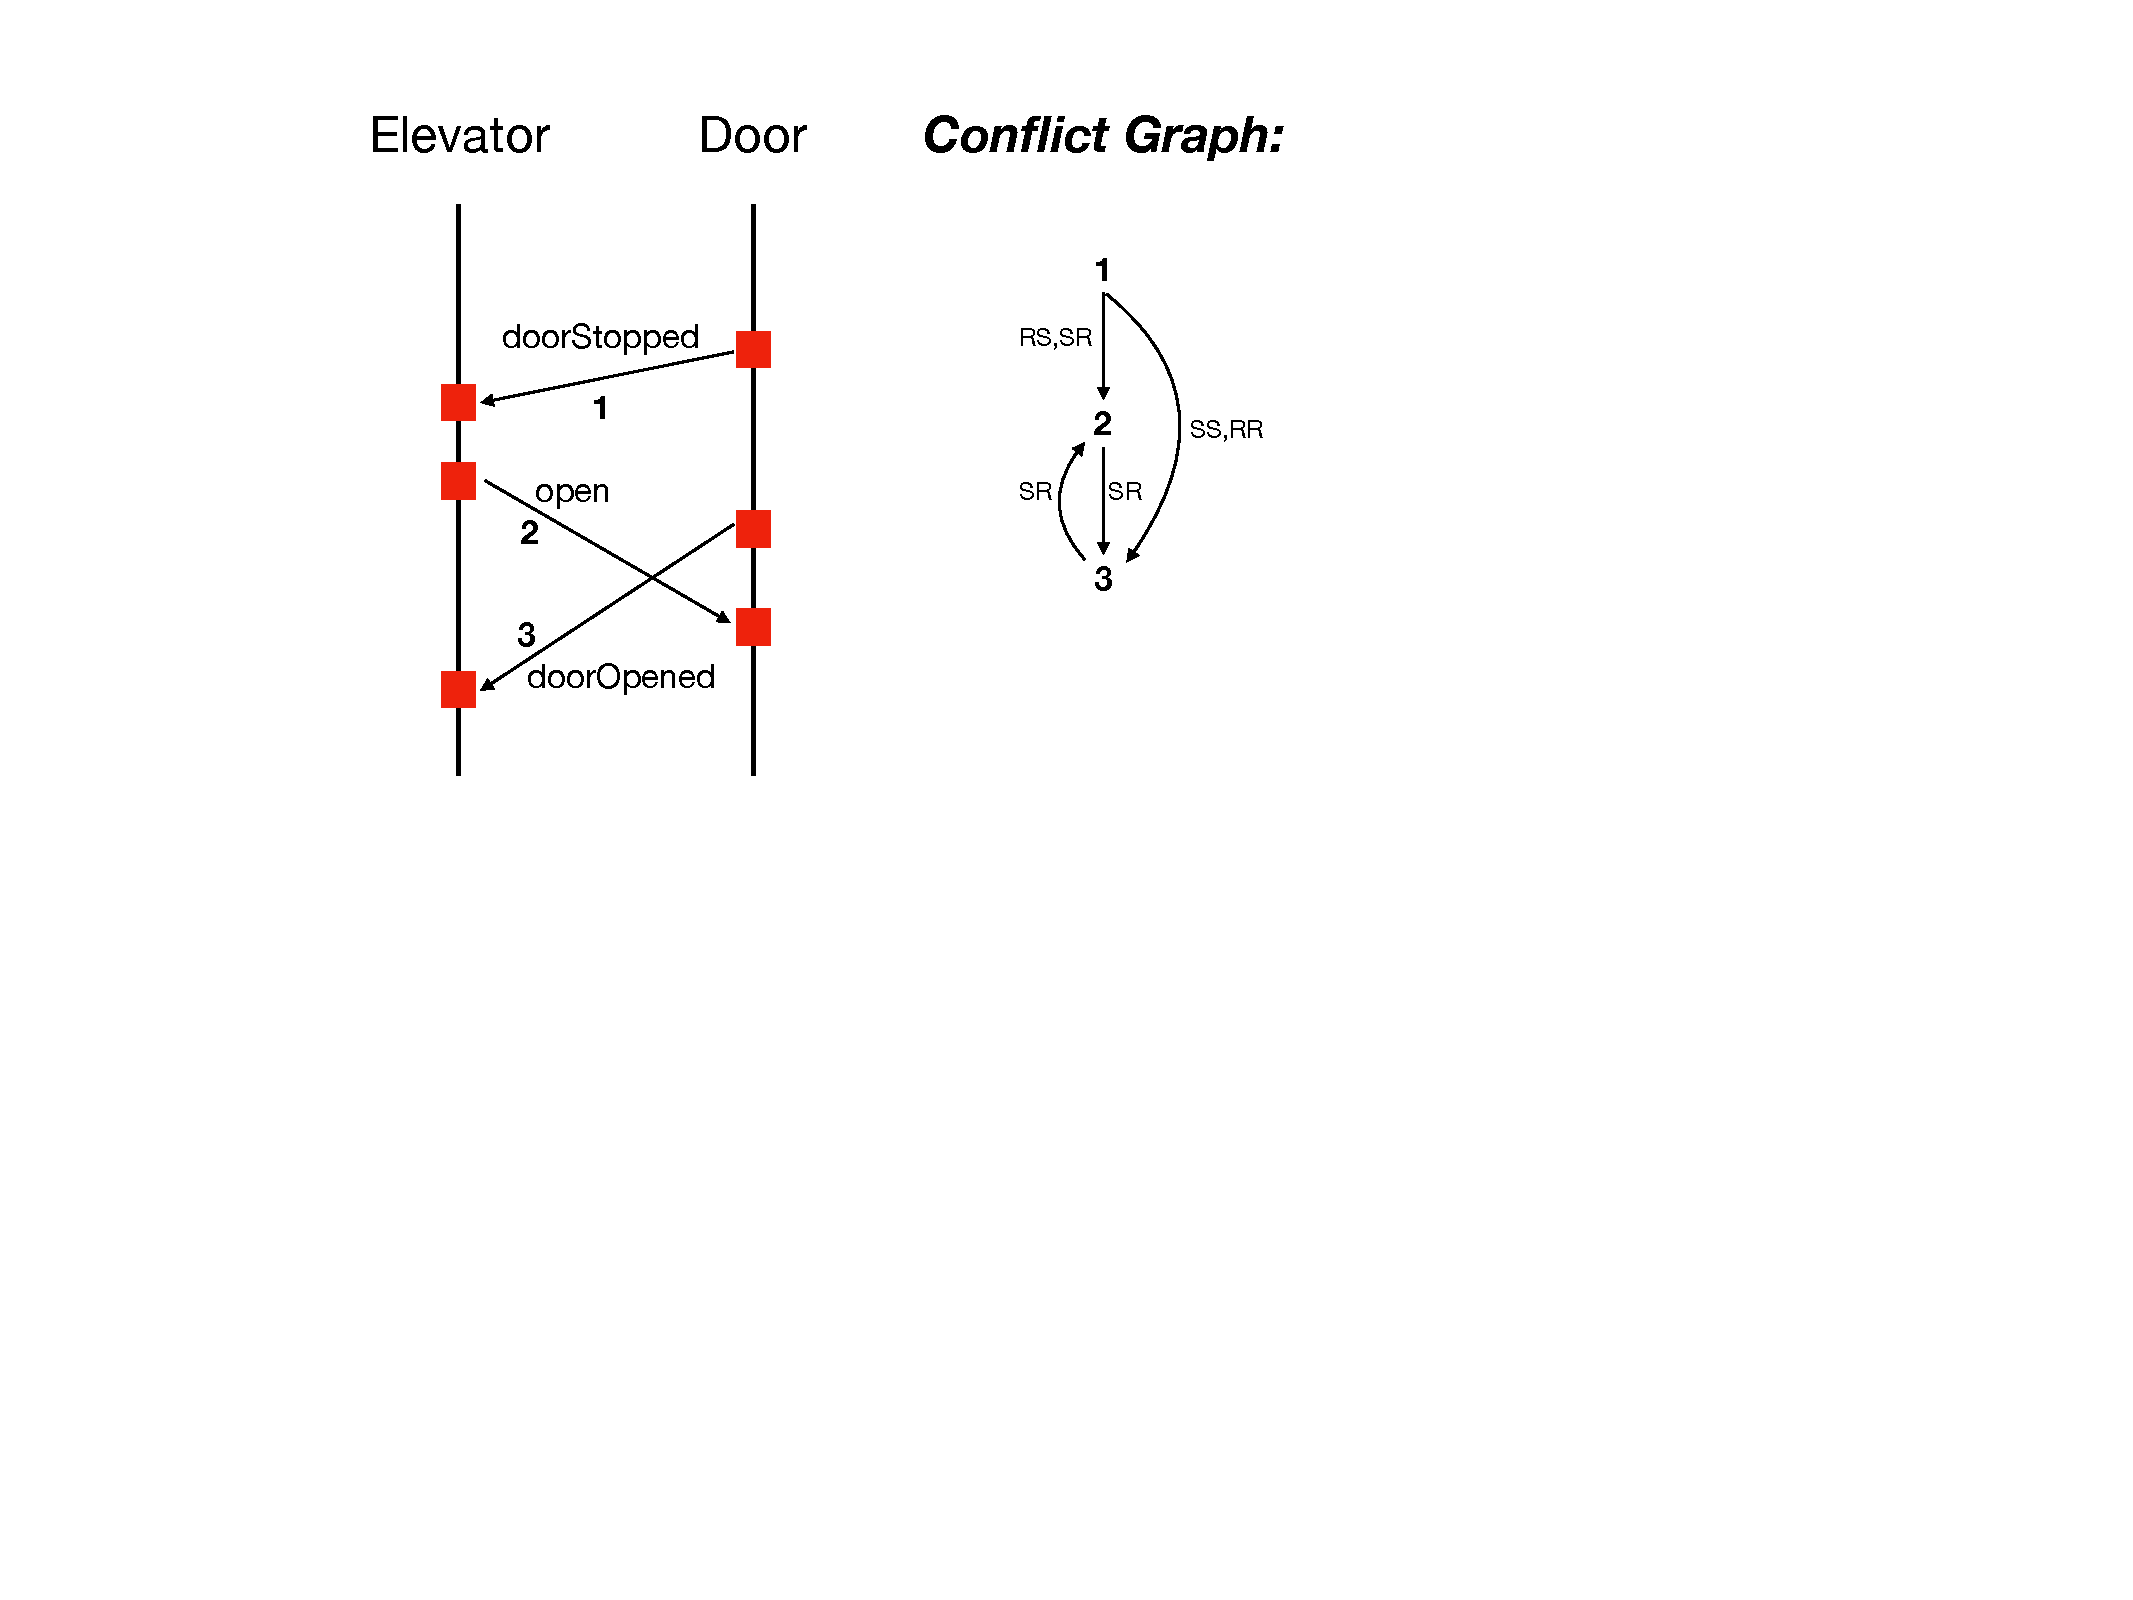
\includegraphics[width=5cm]{MSC-elevator2.pdf}
\vspace{-3mm}
\caption{A computation with a 2-exchange.}
\label{fig:elevator-exec2}
\end{subfigure}
\vspace{-2mm}
\caption{Executions of the Elevator.}
\label{fig:elevator-exec}
\vspace{-6mm}
\end{figure}

%\begin{figure}
%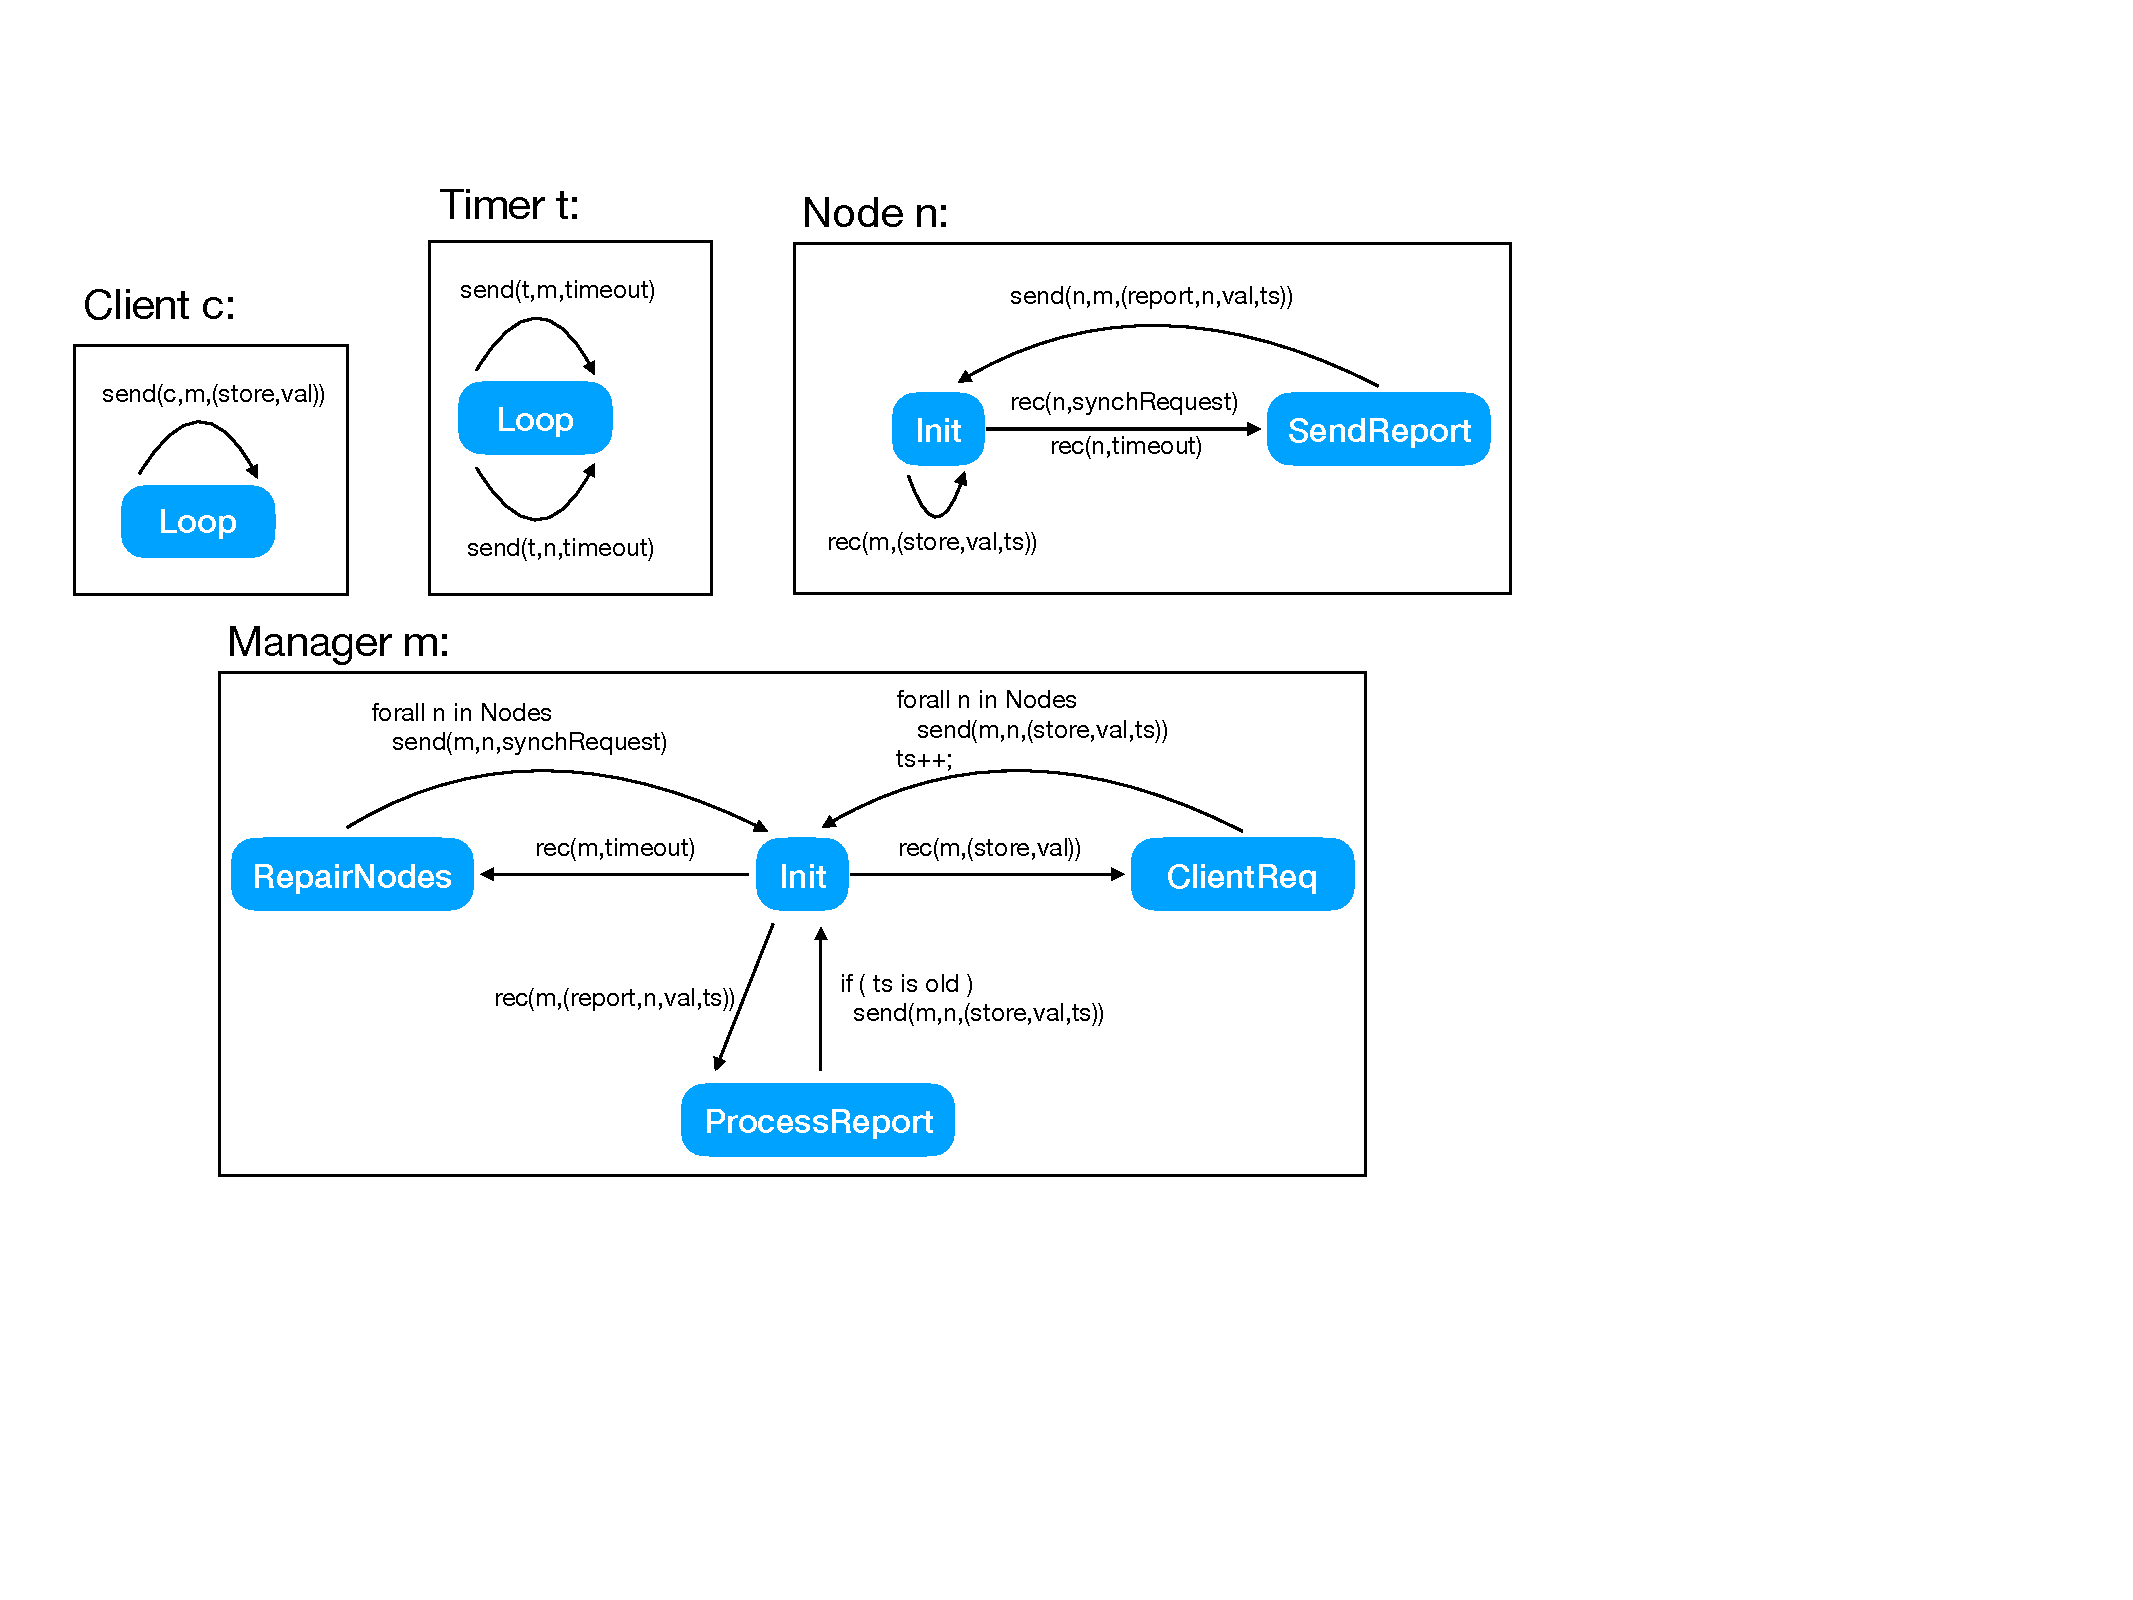
\includegraphics[width=10cm]{replication.pdf}
%\caption{A replication storage protocol}
%\label{fig:replication}
%\end{figure}
%
%\begin{figure}
%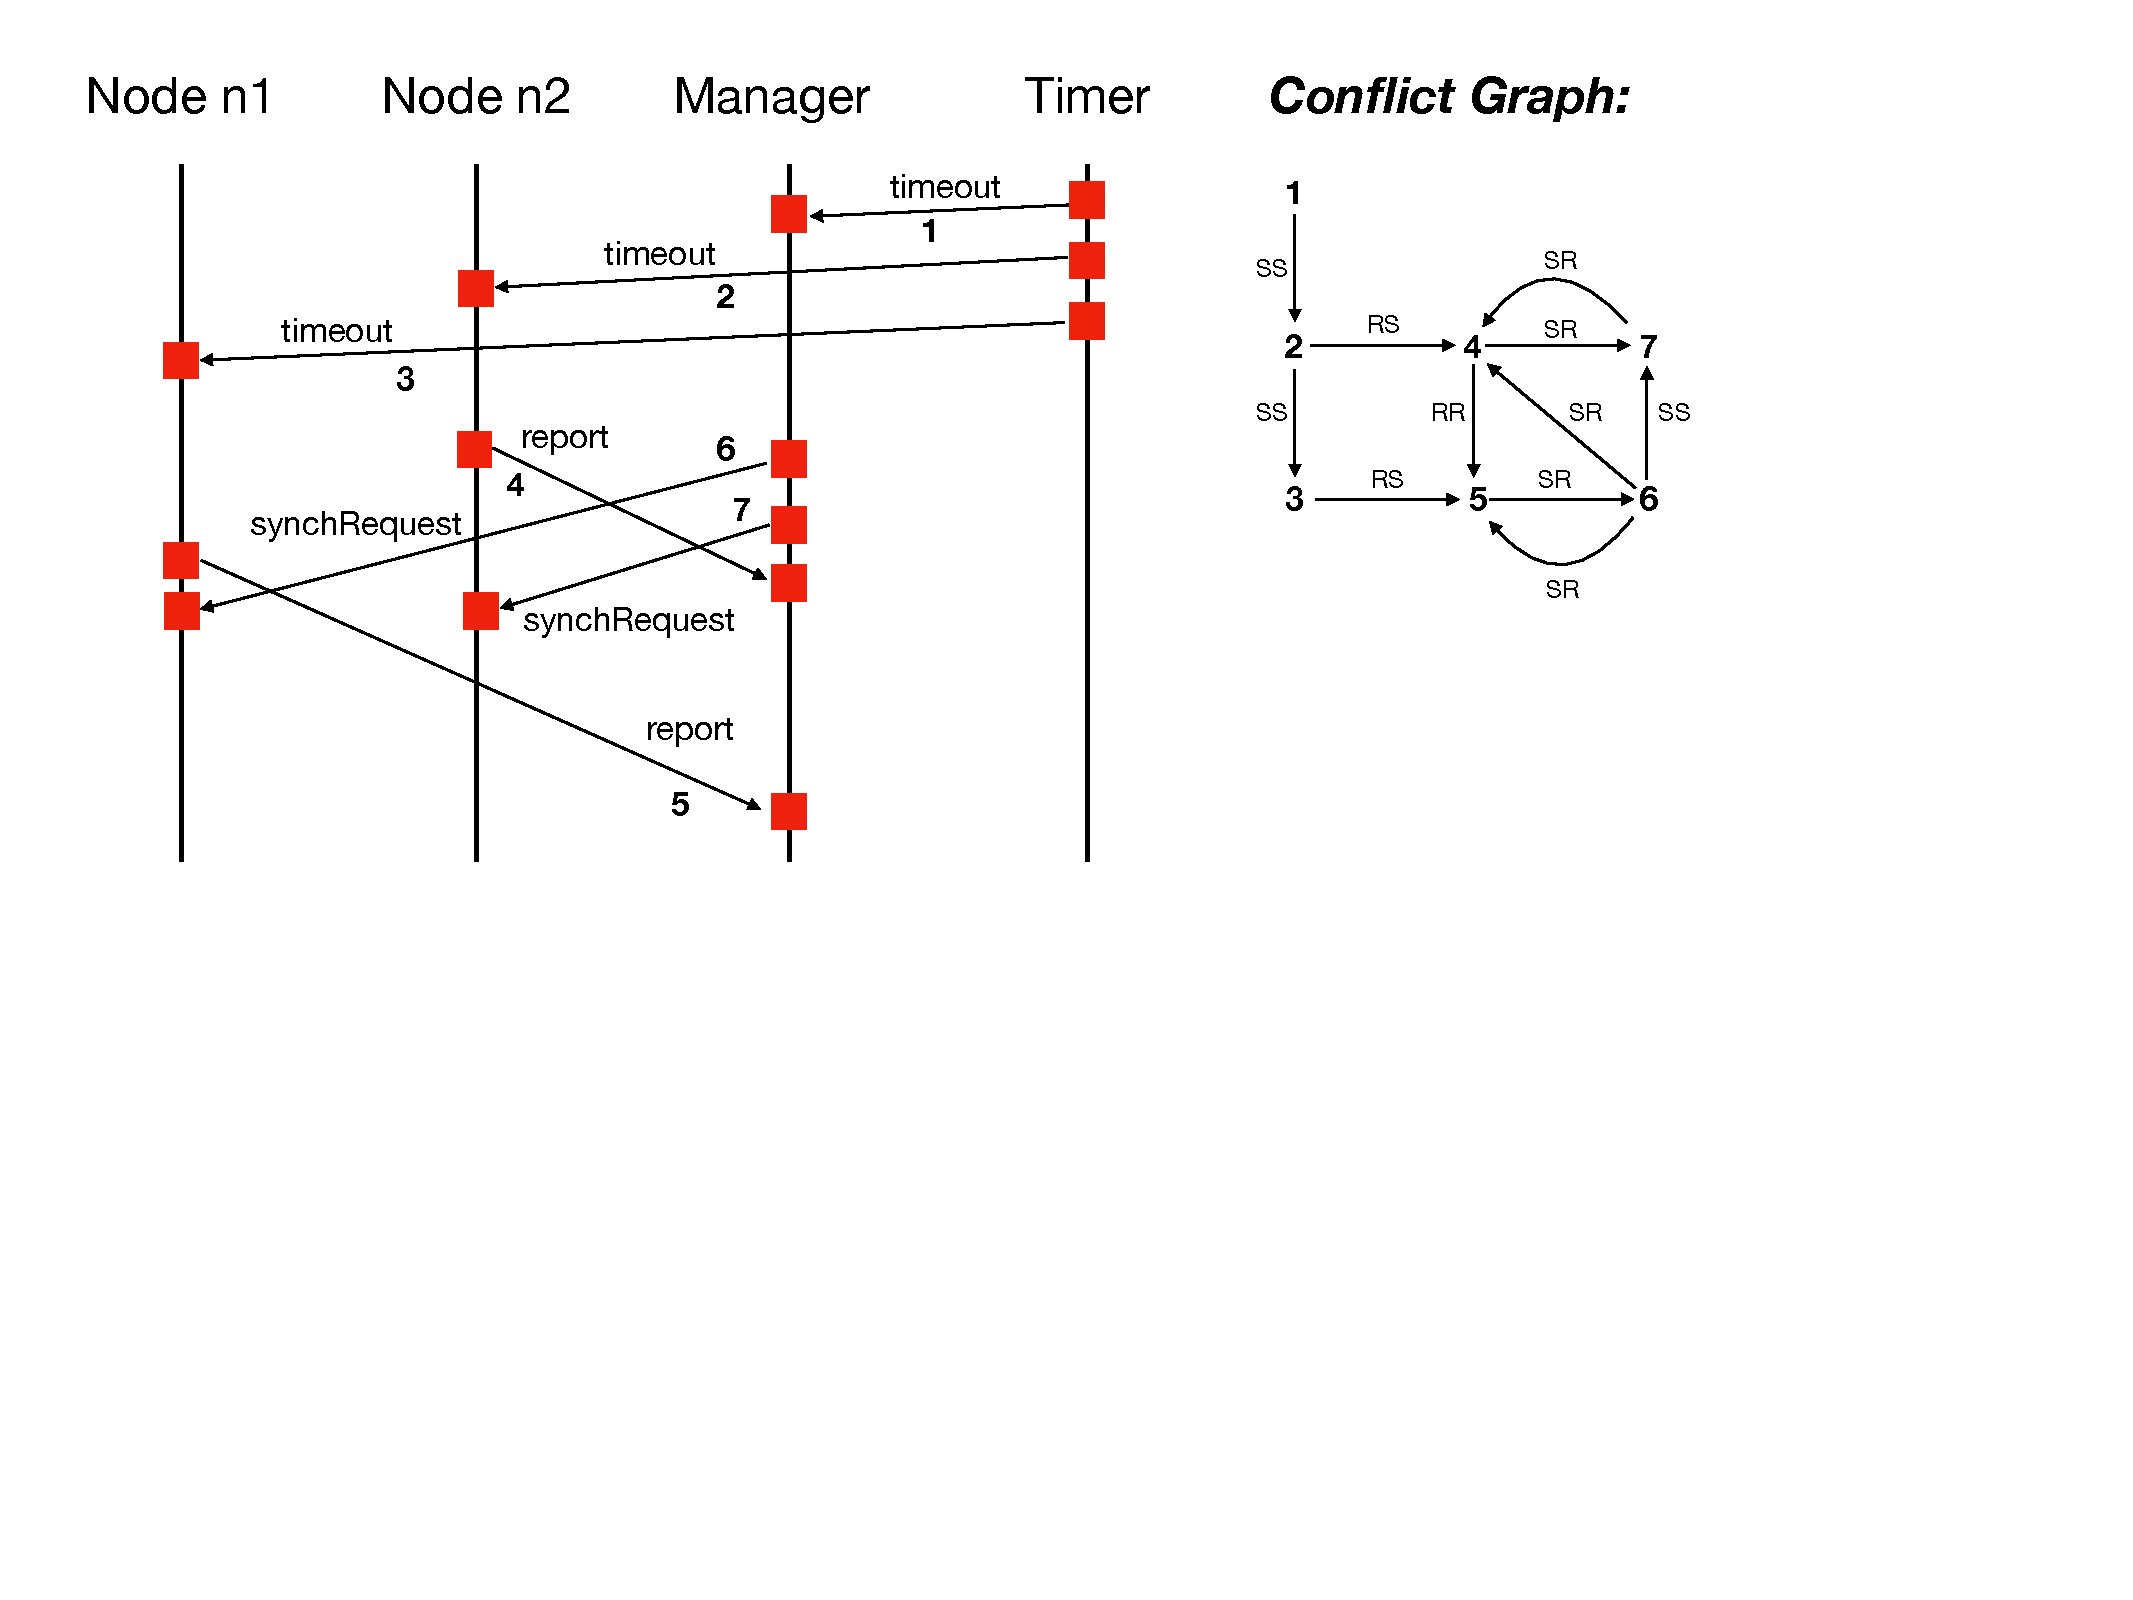
\includegraphics[width=7cm]{MSC-storage.pdf}
%\caption{An execution of the replication storage protocol and its conflict graph.}
%\label{fig:replic-exec}
%\end{figure}



%We have investigated other examples defined in the P language~\footnote{Available at \url{https://github.com/p-org}.}, e.g., a replication storage protocol (see Appendix~\ref{asec:motivation}), an implementation of the German cache coherence protocol and an implementation of a device driver, and we have established manually and through testing that they are $k$-synchronizable~\footnote{For the testing part, we have checked on tens of thousands of executions generated through randomized testing, each execution with thousands of steps, that the corresponding conflict-graph satisfies the properties required for $k$-synchronizability.}. The value of $k$ is most of the times $1$ or $2$.

%\cite{PRuntime}

%\begin{figure}
%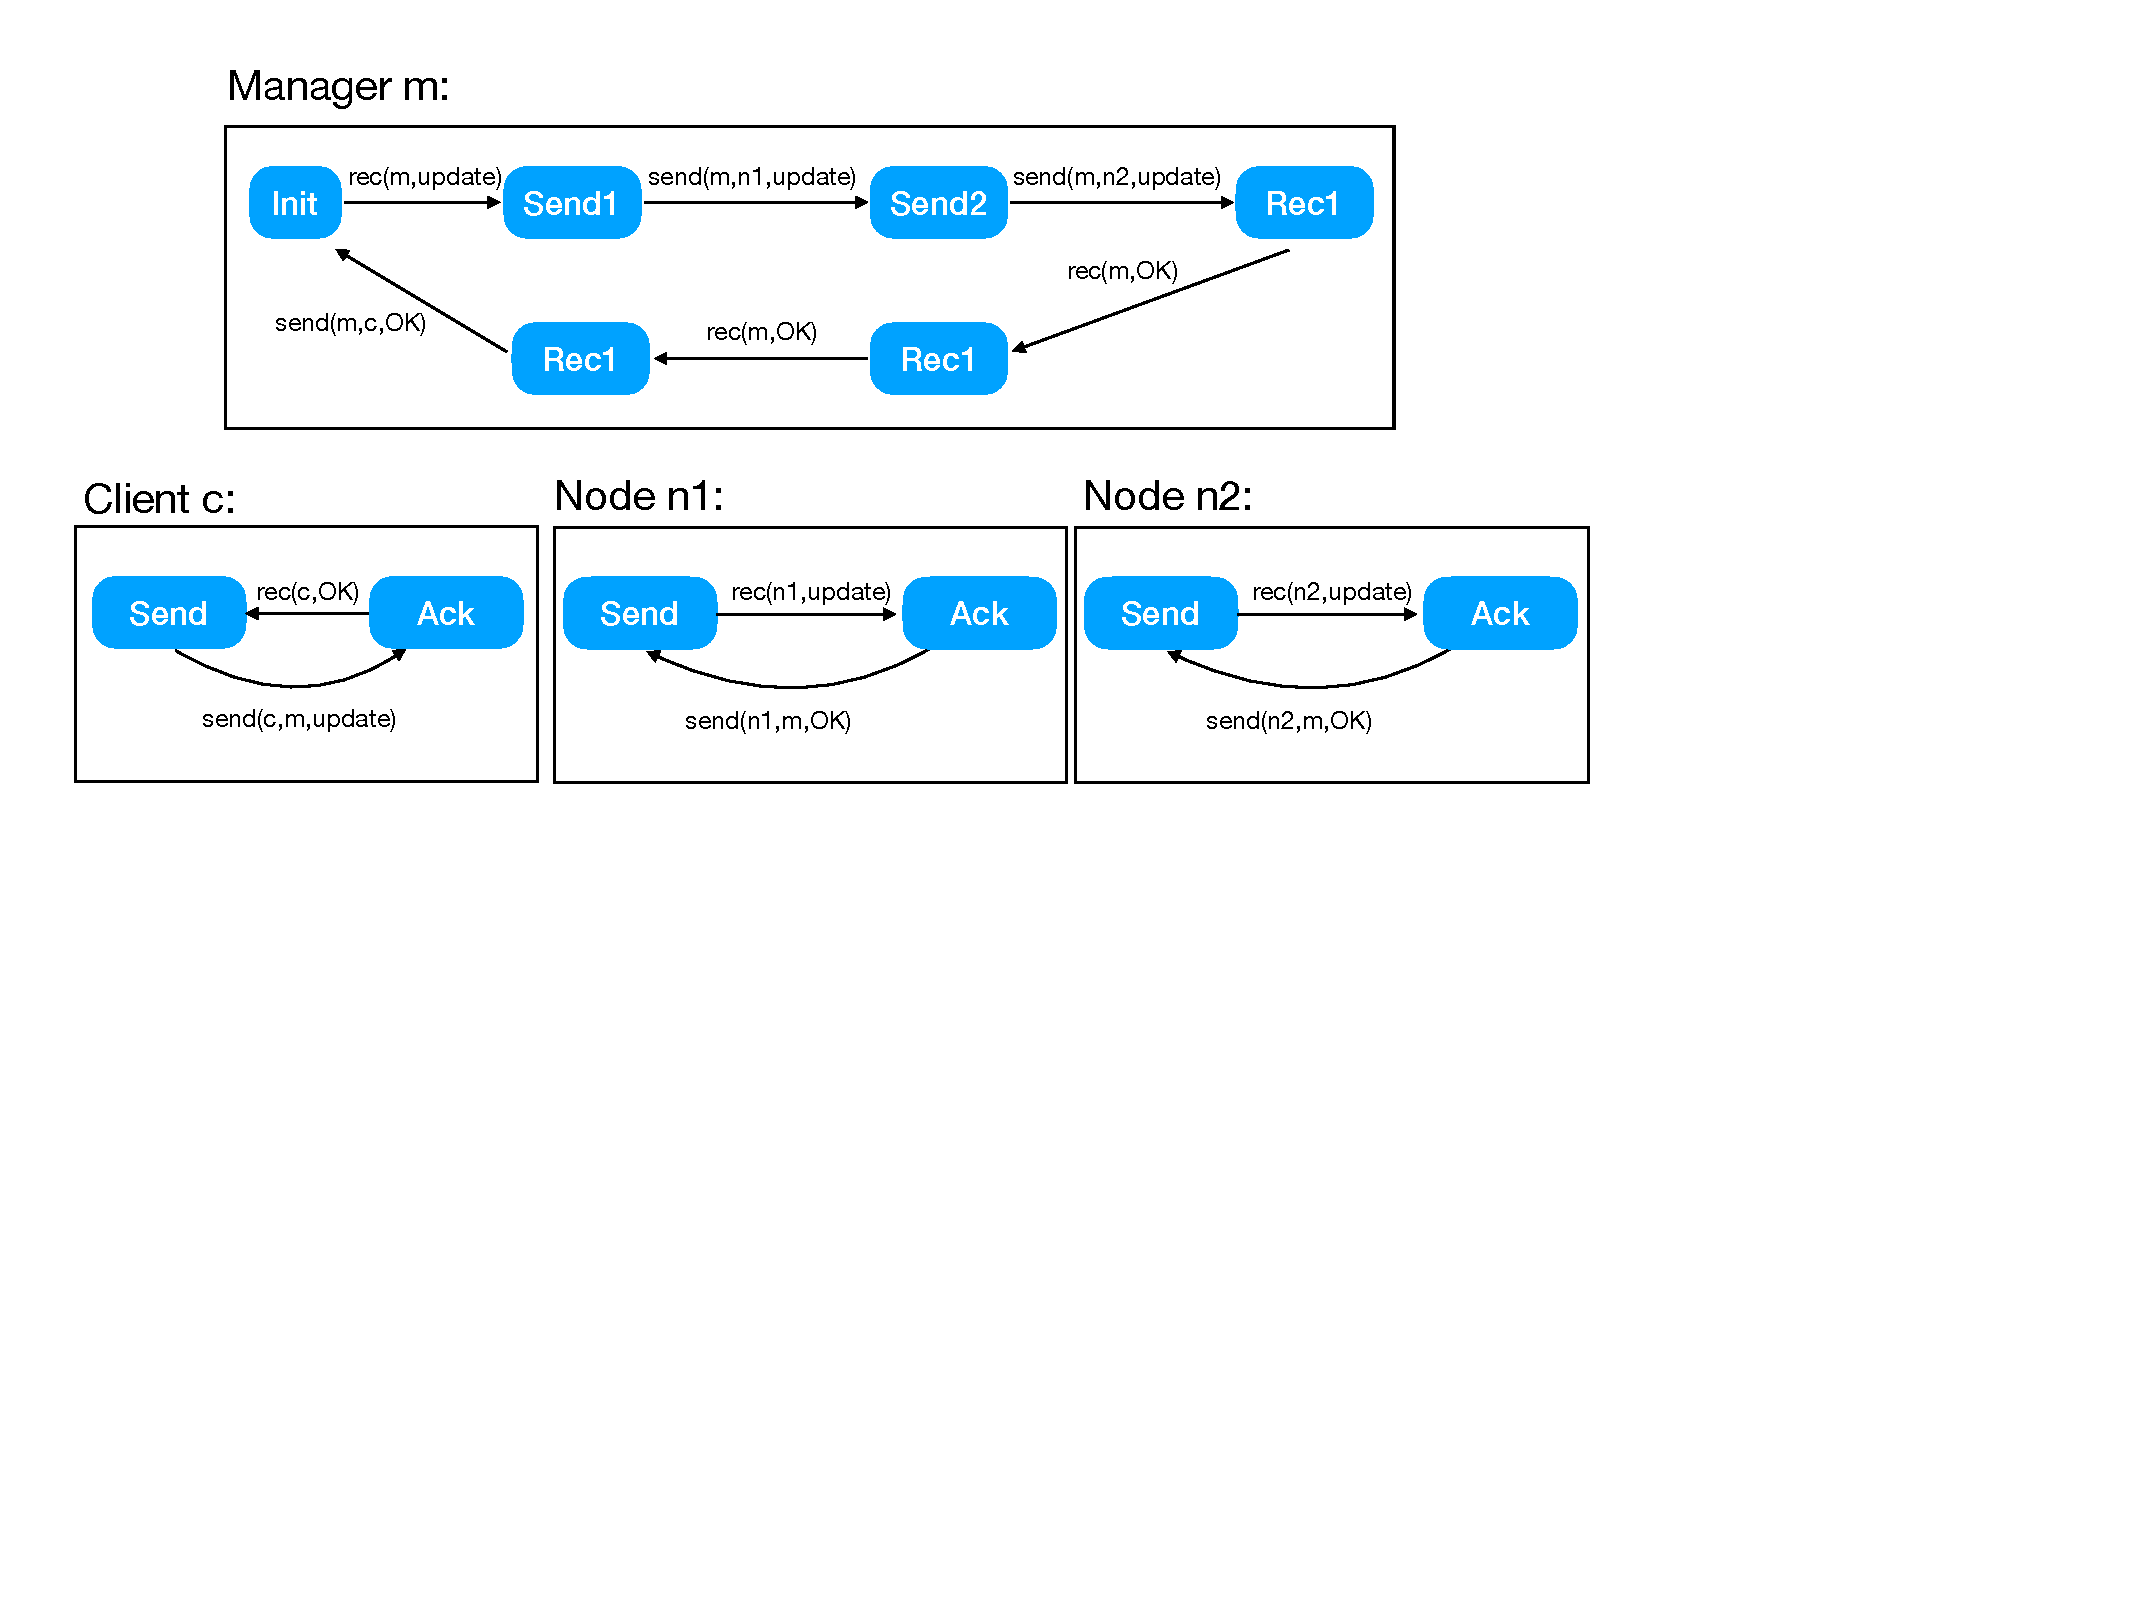
\includegraphics[width=10cm]{commit.pdf}
%\caption{A distributed commit protocol.}
%\label{fig:commit}
%\end{figure}
%
%\begin{figure}
%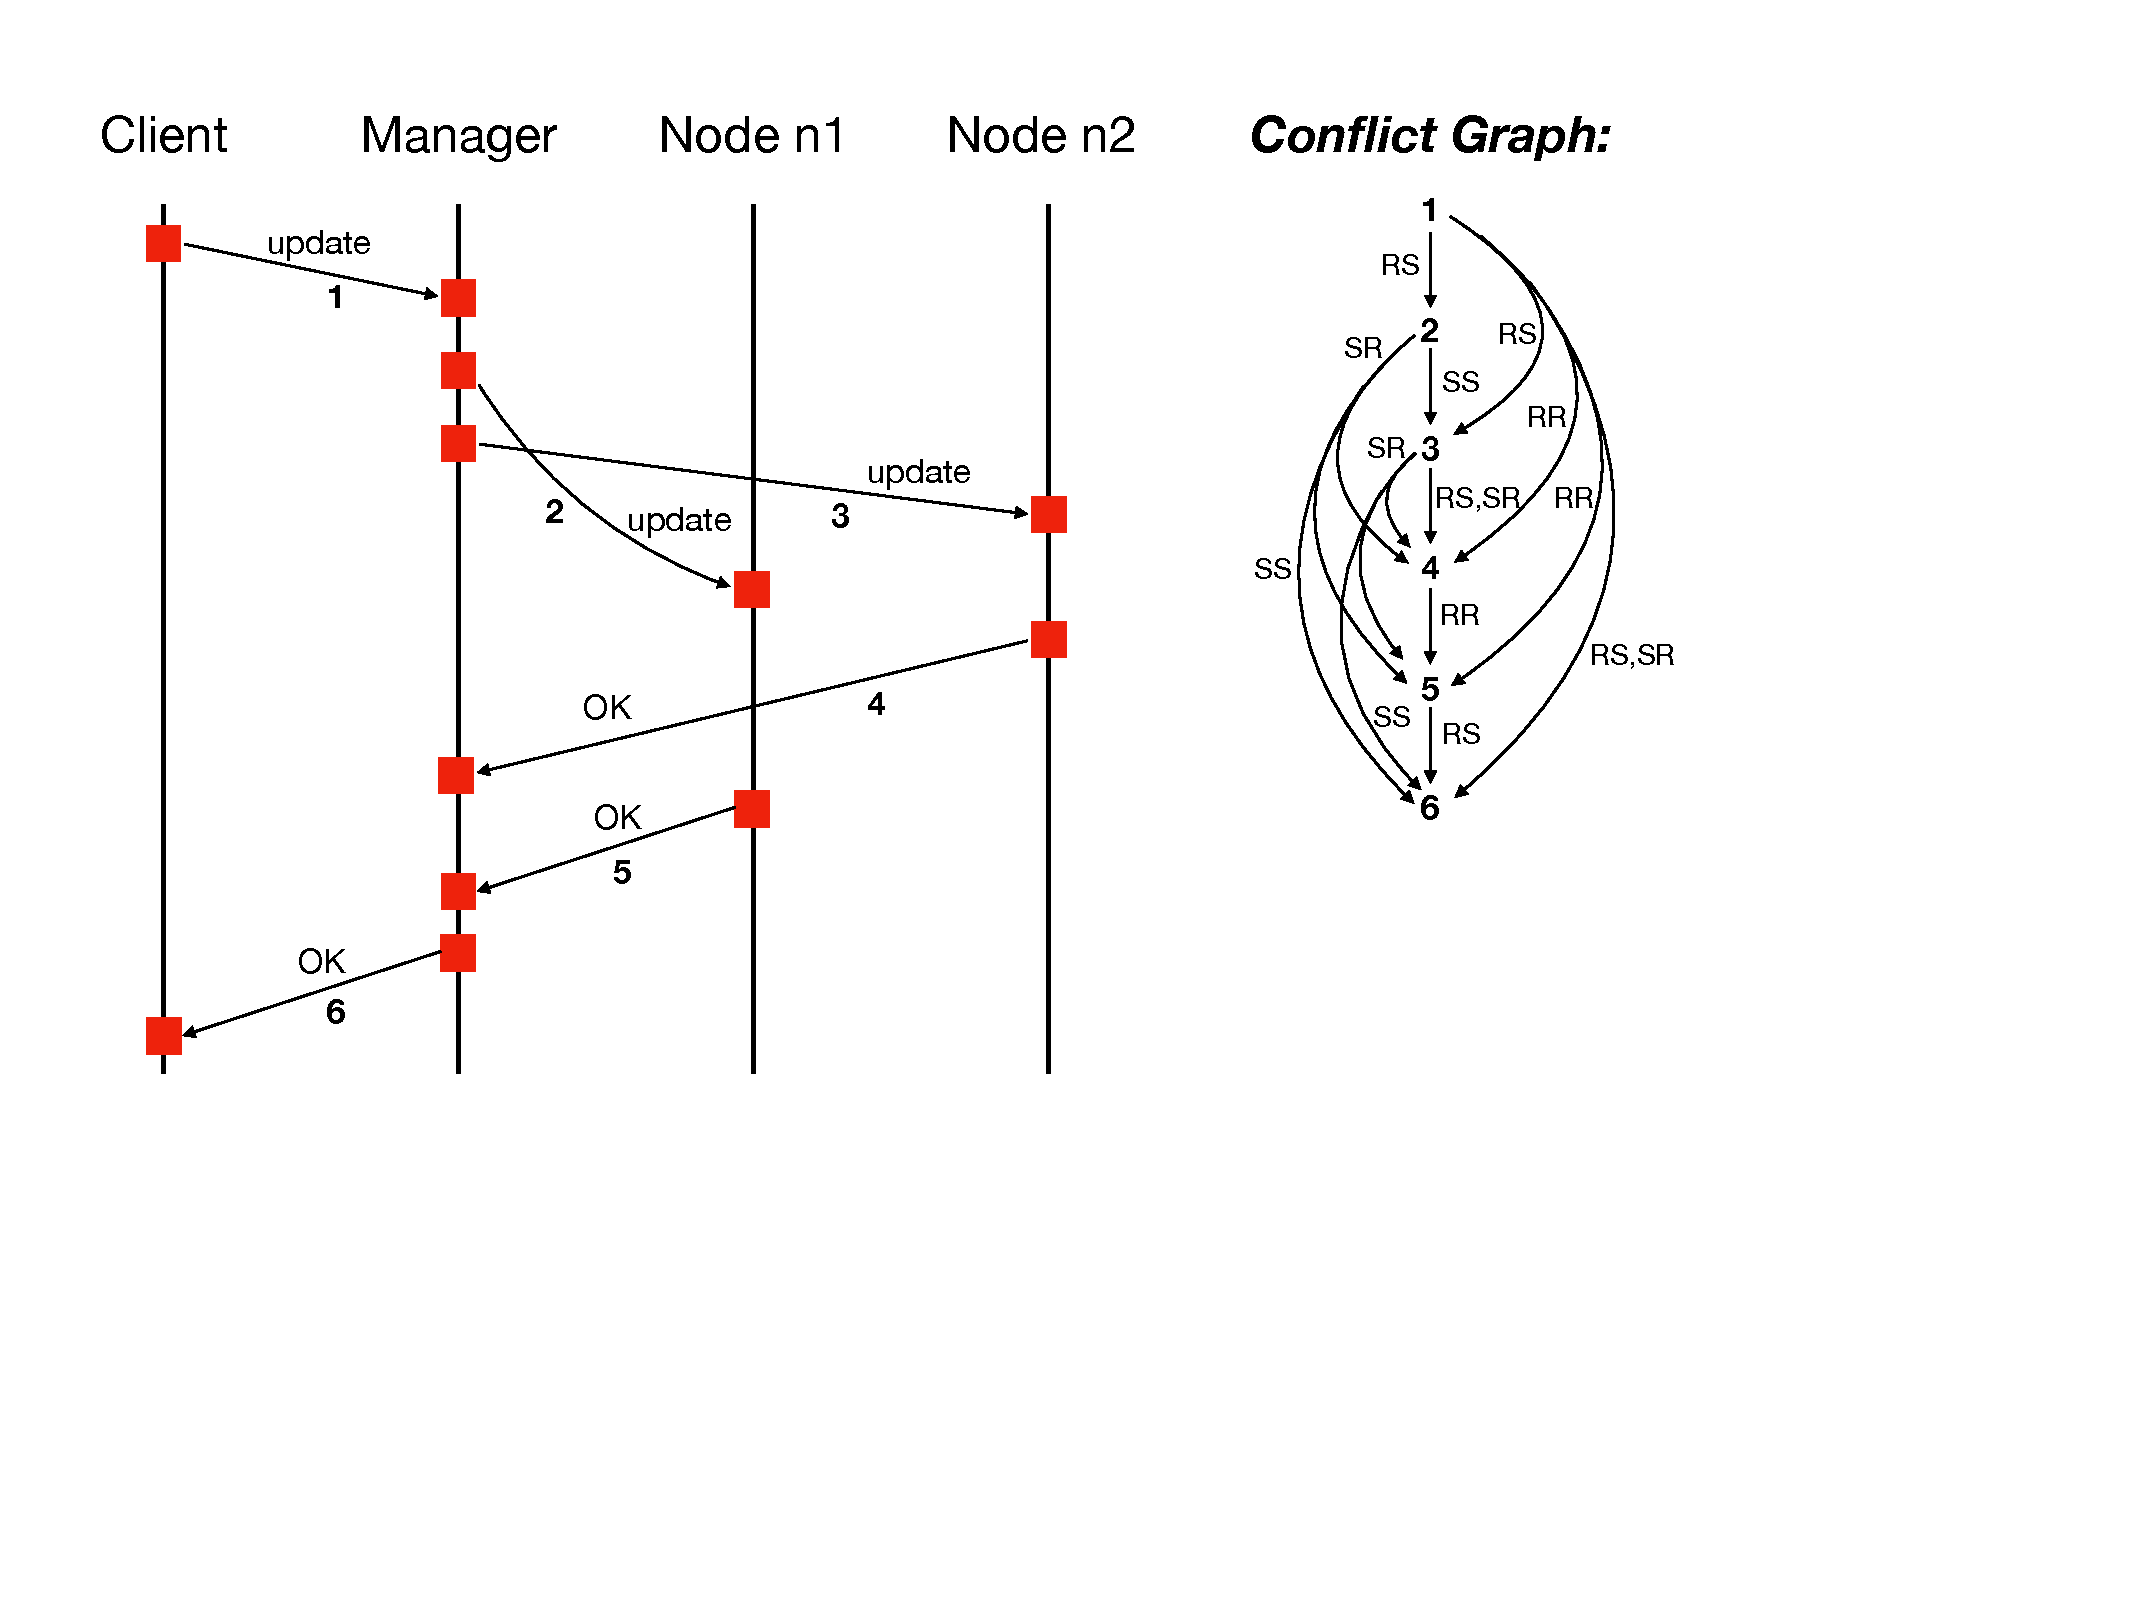
\includegraphics[width=7cm]{MSC-commit.pdf}
%\caption{An execution of the distributed commit protocol and its conflict graph.}
%\label{fig:commit-exec}
%\end{figure}

%\begin{figure}
%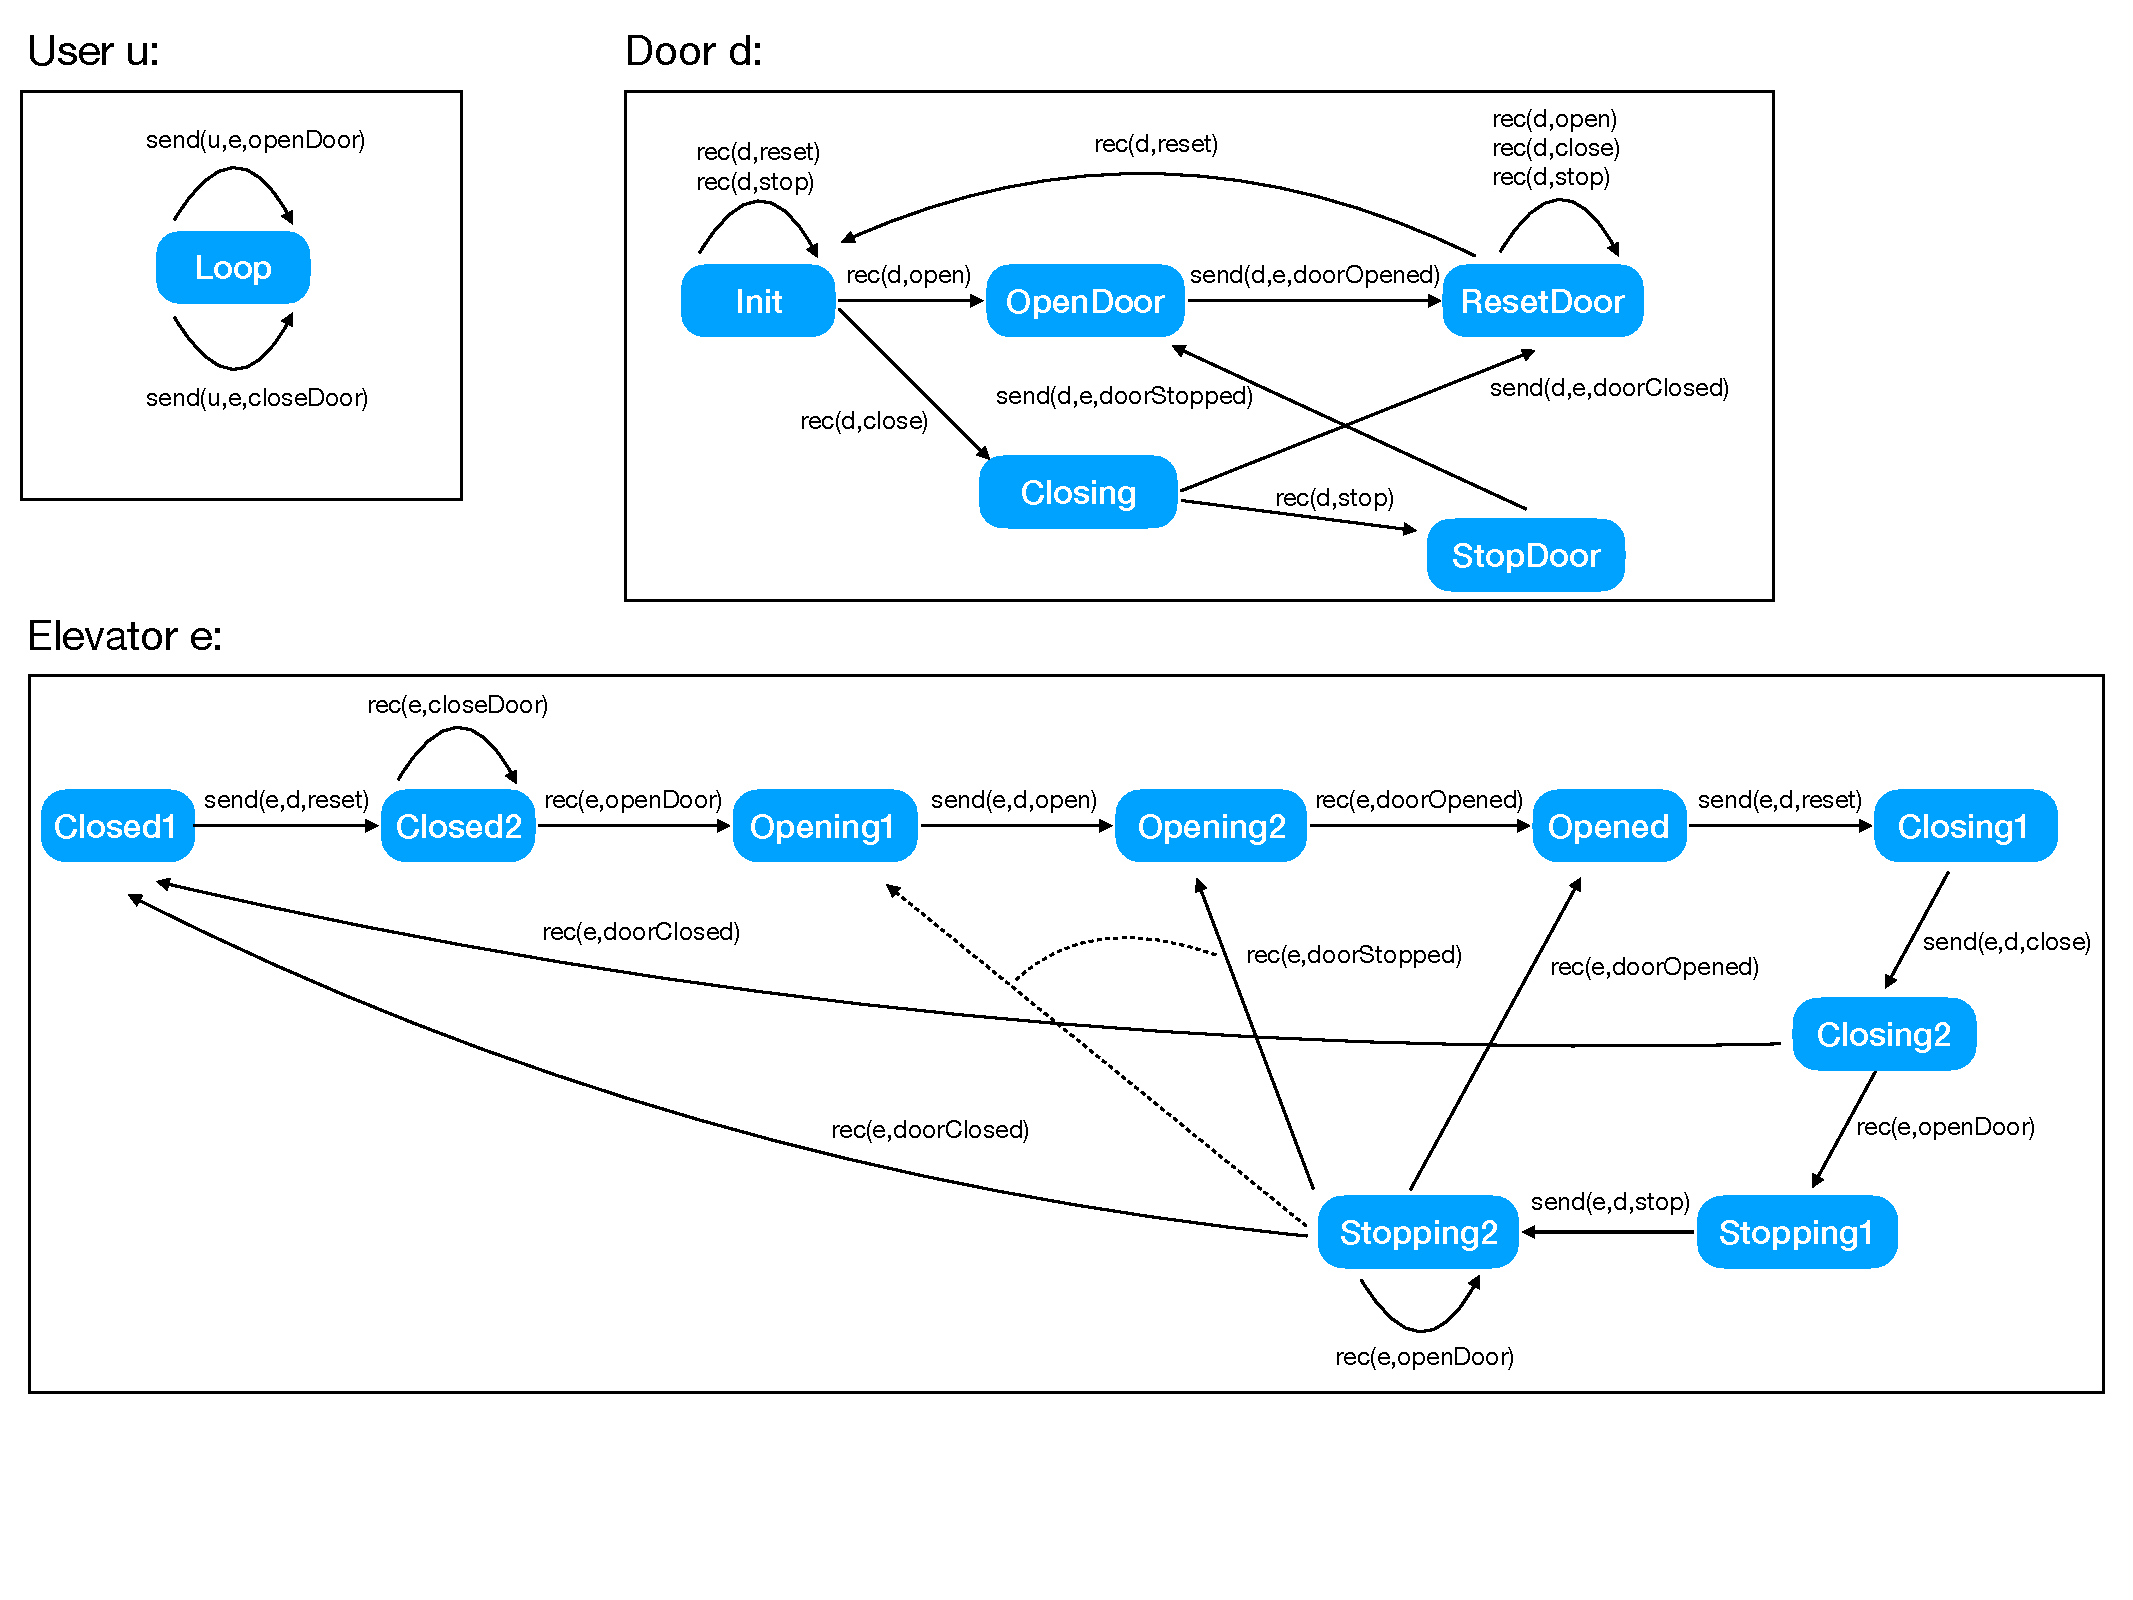
\includegraphics[width=13cm]{elevator.pdf}
%\caption{The Elevator example}
%\label{fig:elevator}
%\end{figure}
%
%\begin{figure}
%\begin{subfigure}[t]{6cm}
%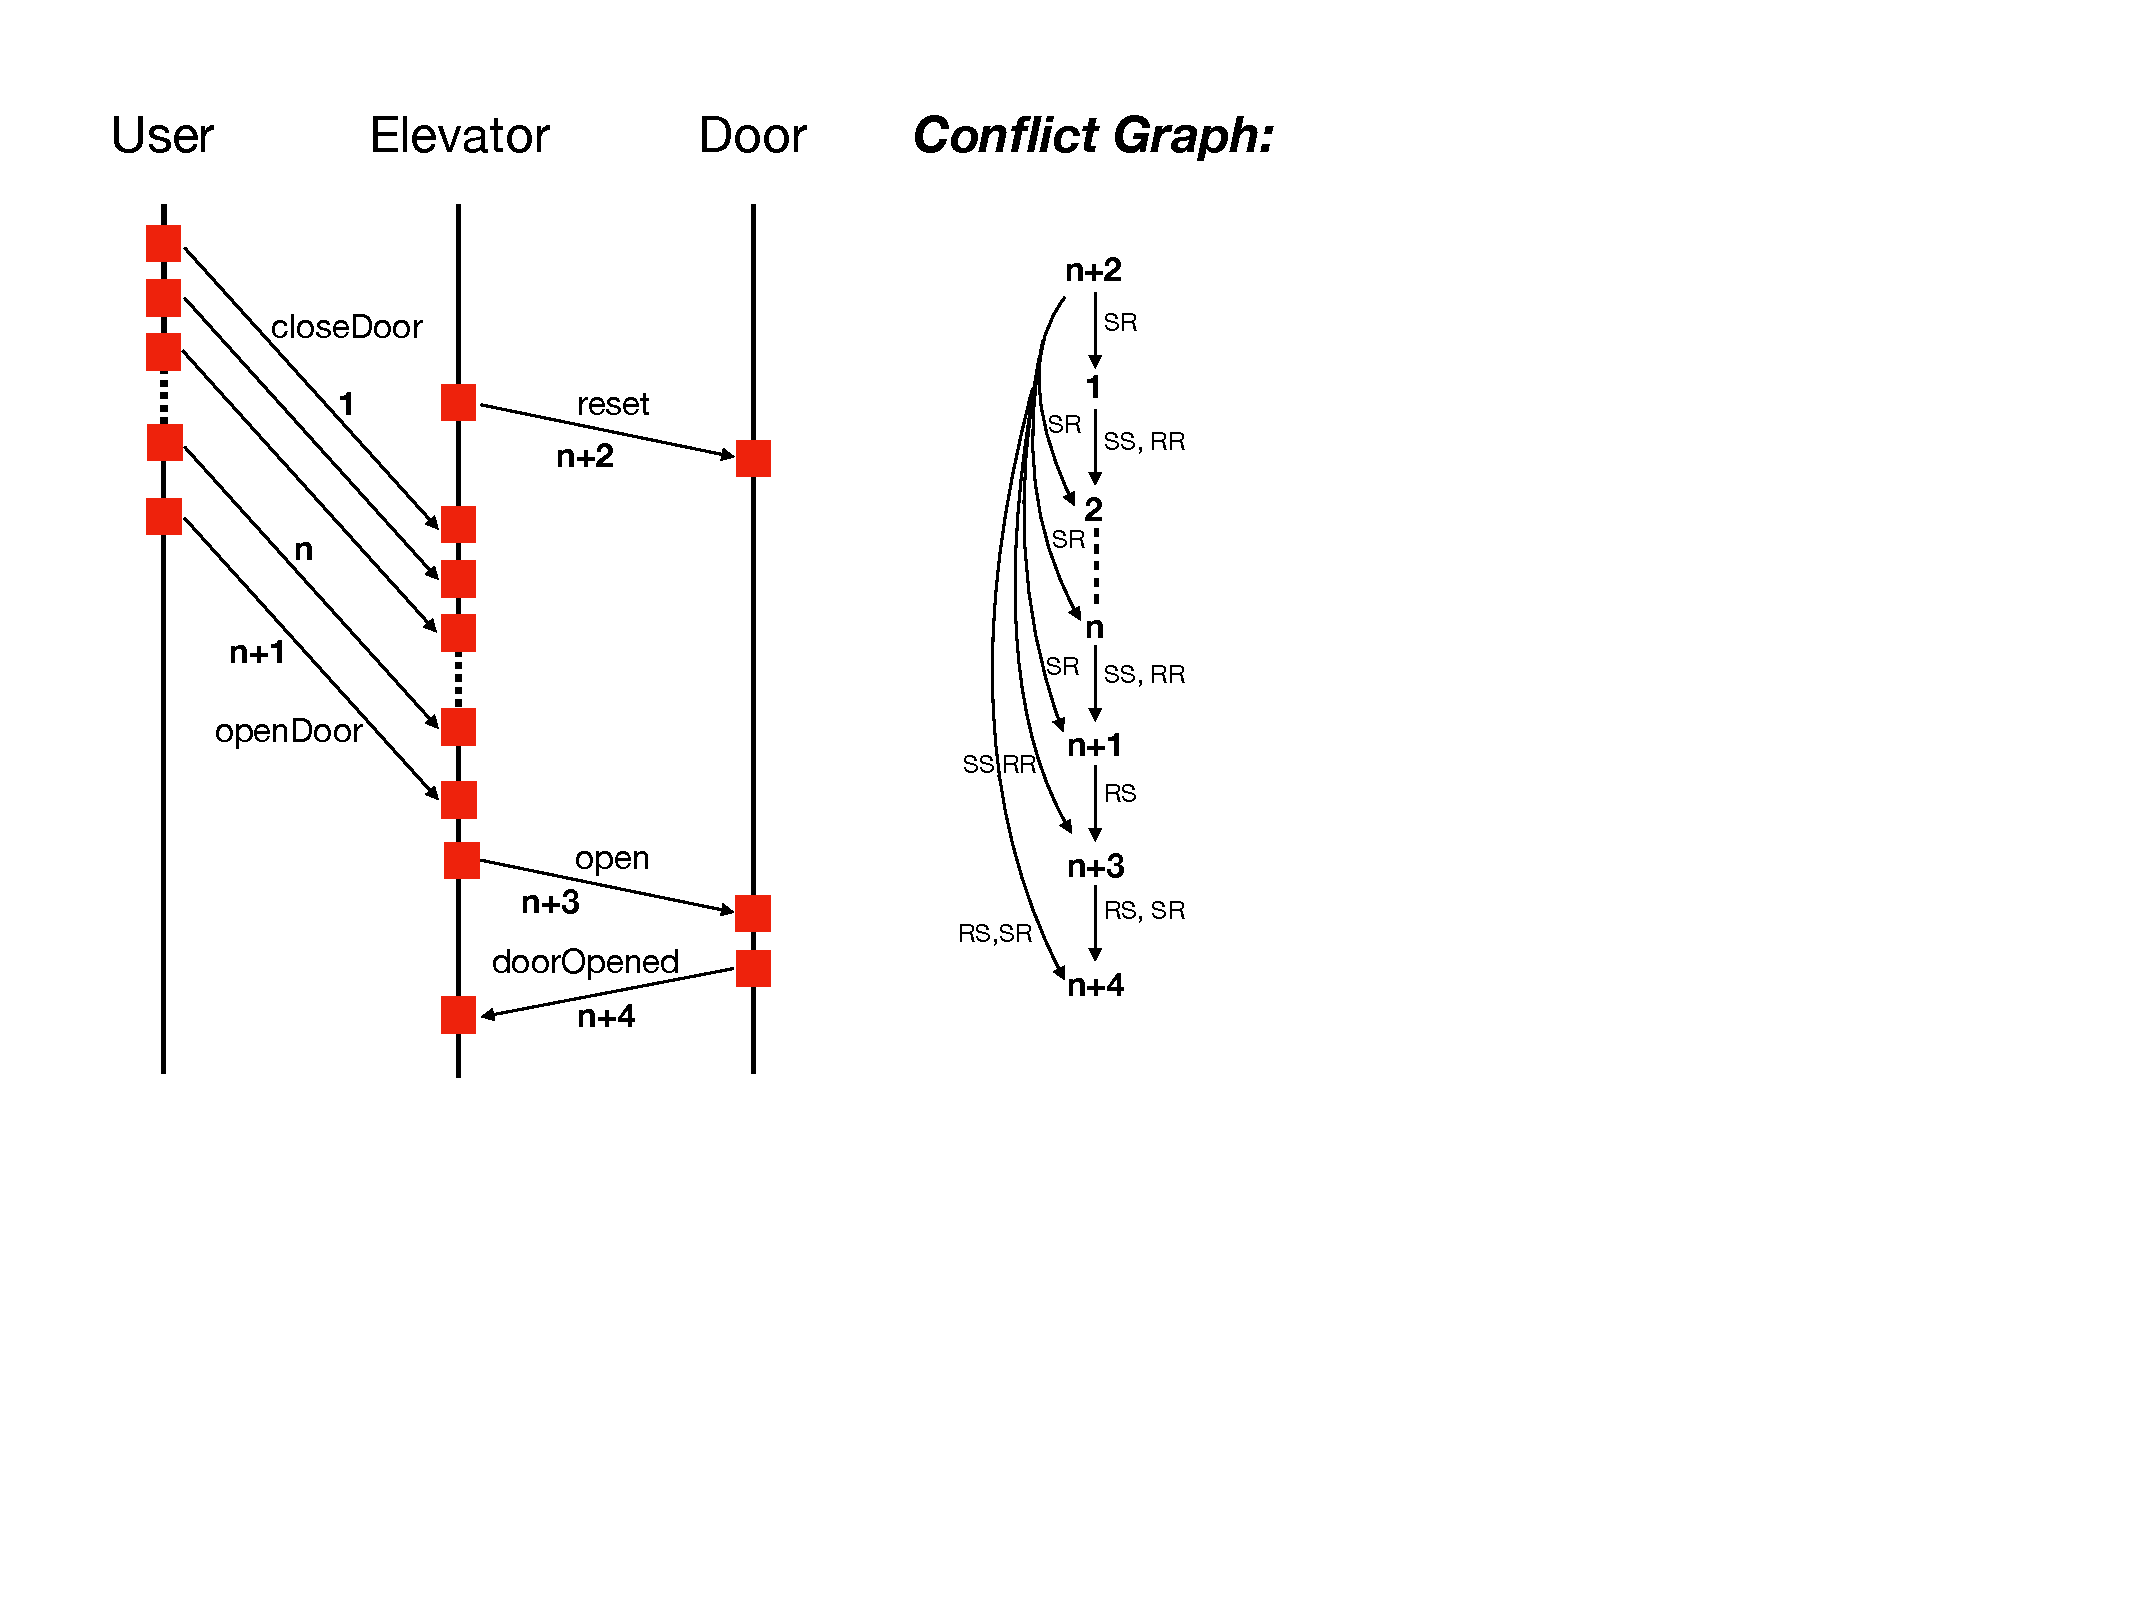
\includegraphics[width=6cm]{MSC-elevator1.pdf}
%\caption{A synchronizable execution.}
%\label{fig:elevator-exec1}
%\end{subfigure}
%\hspace{1cm}
%\begin{subfigure}[t]{5cm}
%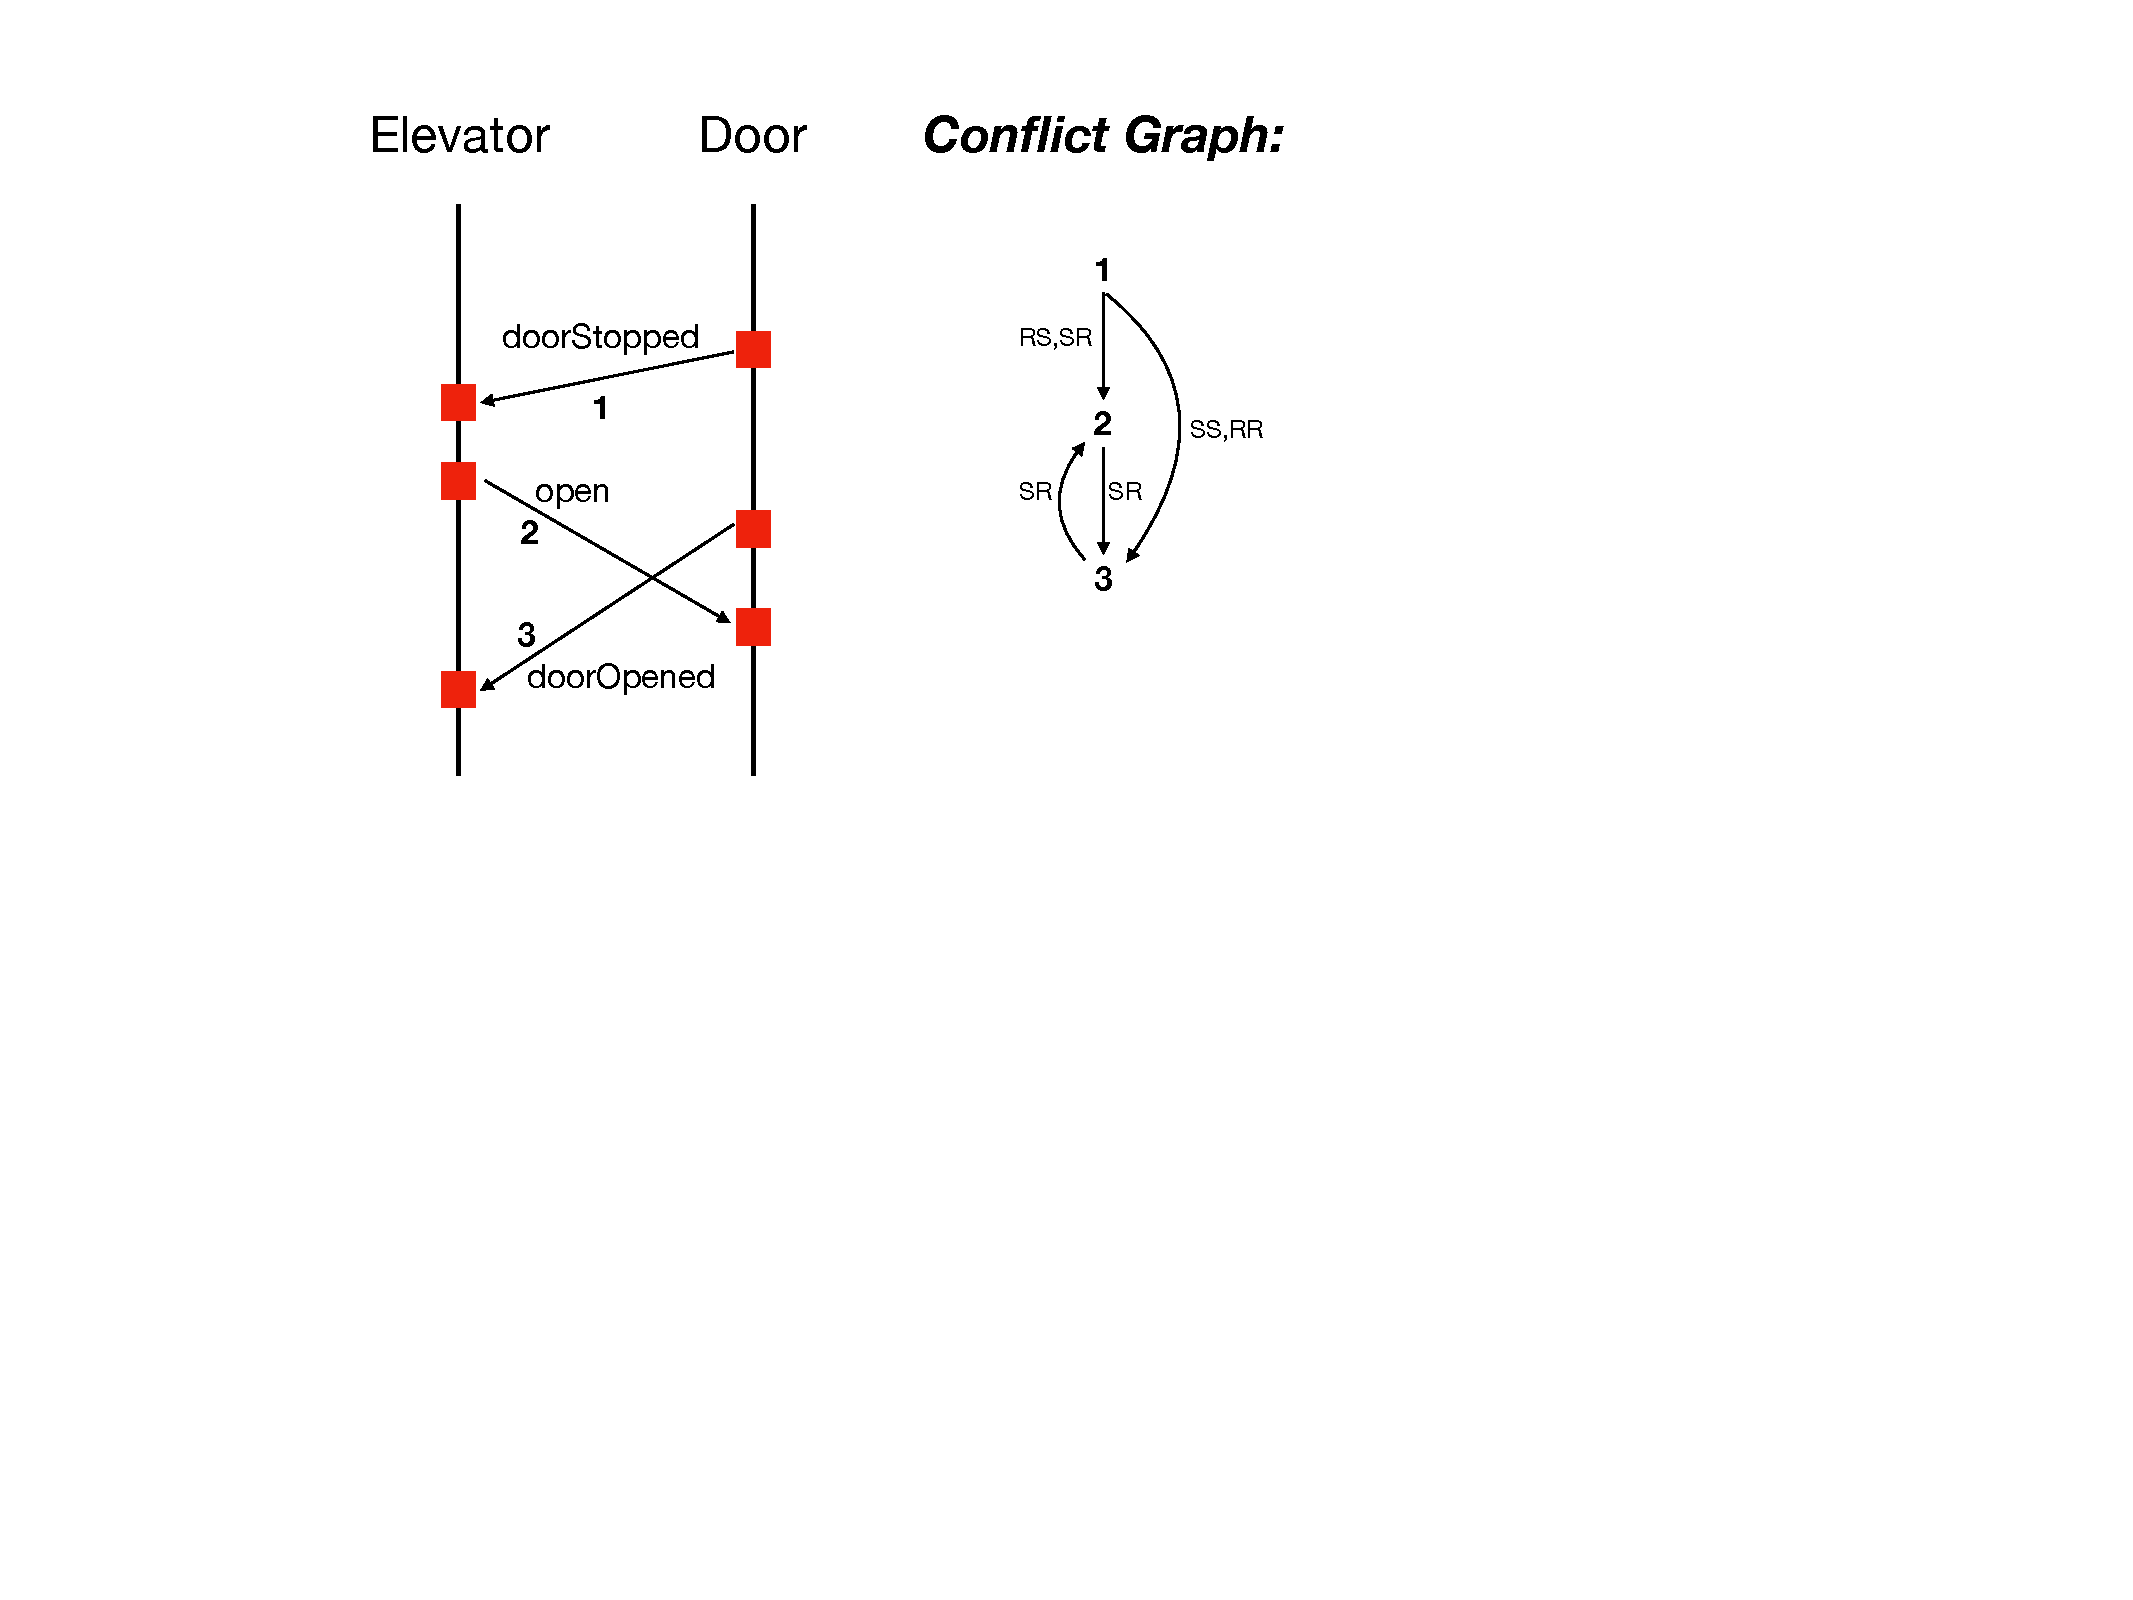
\includegraphics[width=5cm]{MSC-elevator2.pdf}
%\caption{A computation with a 2-exchange.}
%\label{fig:elevator-exec2}
%\end{subfigure}
%\caption{Executions of the elevator.}
%\label{fig:elevator-exec}
%\end{figure}

